\chapter{DESENVOLVIMENTO} \label{cap:desenvolvimento}

Neste capítulo, serão descritos alguns detalhes da construção dos métodos e do algoritmo para avaliação de sua performance, além disso, serão mostradas as dificuldades encontradas na aplicação prática desses métodos. A discretização da estimação de densidades de variáveis discriminantes pode influenciar de forma direta na tarefa de classificação, entretanto, este trabalho se concentrou somente no impacto desses métodos na estimação, entendendo que um menor erro de estimação pode levar a uma melhor classificação.

\section{Conjunto de dados}

Um dos objetivos desse trabalho é otimizar o desempenho dos algoritmos de estimação de densidade via KDE que fazem uso de métodos de discretização e posteriormente essas estimações serão usadas para a identificação e classificação de eventos. Portanto o conjunto de dados aqui escolhido tem por base as estimações que podem ser encontradas em alguns dos experimentos de física de partículas mais importantes atualmente, como o ATLAS e CMS.

Nas Figuras \ref{fig:15} e \ref{fig:16} são mostrados casos representativos de variáveis usadas para a identificação de elétrons nos experimentos CMS e ATLAS, respectivamente. Para o CMS, pode-se ver o perfil dos elétrons e do ruído de fundo, bem como a diferença entre dados reais e simulados. Já na Figura \ref{fig:16} é mostrado também as varias formas de ruído de fundo para elétrons no ATLAS.


\begin{figure}[H]
	\begin{center}
		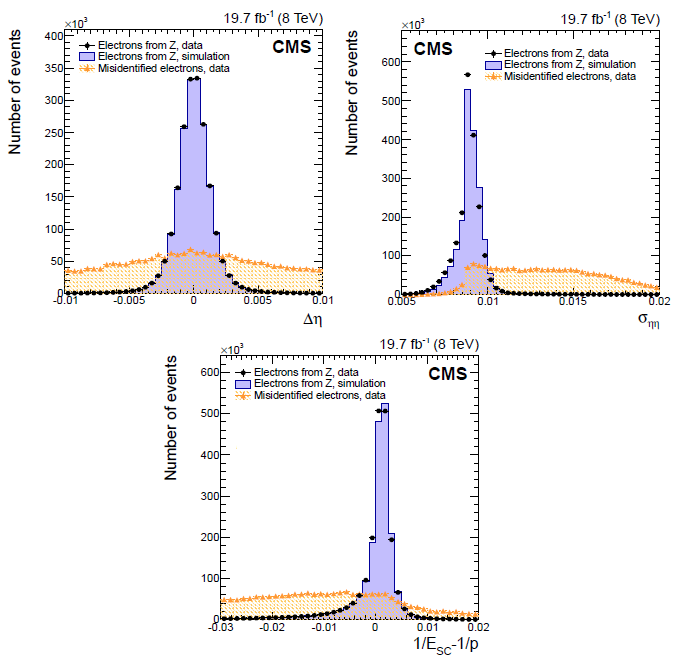
\includegraphics[width=0.8\linewidth]{./figuras/variaveisCMS.png}
		\caption{Caso representativo, variáveis de identificação de elétrons, do experimento CMS: variável $\Delta\eta$, forma do chuveiro $\sigma_{\eta\eta}$ e distribuição de energia-momento $1/E_{SC}-1/p$. Extraído de \cite{cms2015performance}.}\label{fig:15} 
	\end{center}
\end{figure}

Pode-se considerar que a identificação de elétrons em experimentos de física de altas energias é de certa forma similar, respeitando as particularidades de cada detector. Portanto, é de se esperar que a otimização de algoritmos de identificação de elétrons estudada em um conjunto de dados possa ser reproduzida, considerando as especificidades de cada experimento, em um outro conjunto de dados, fazendo com que o estudo para melhoria do desempenho desse processo seja de suma importância.

\begin{figure}[H]
	\begin{center}
		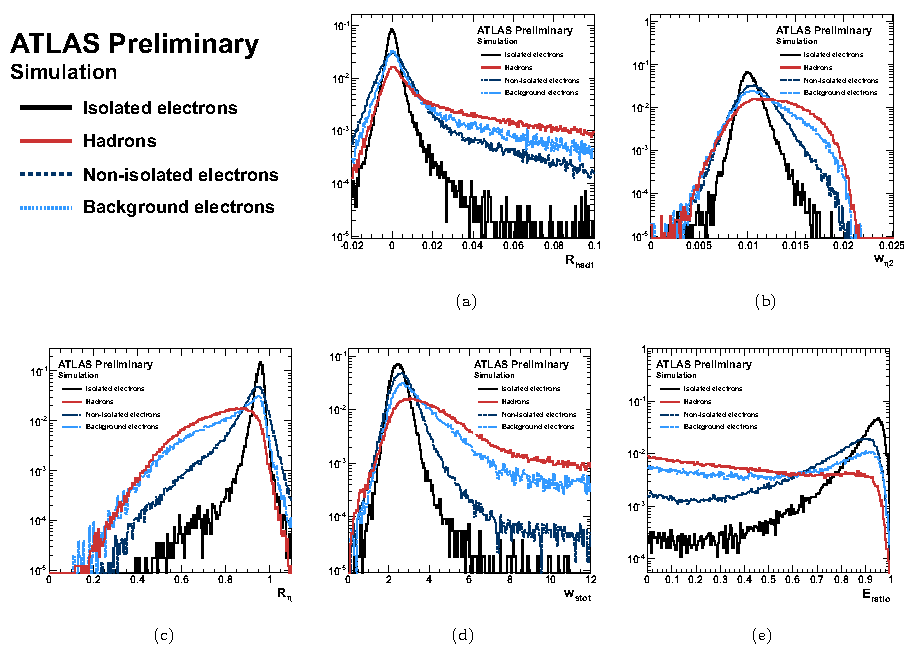
\includegraphics[width=0.8\linewidth]{./figuras/variaveisATLAS.pdf}
		\caption{Caso representativo, variáveis de identificação de elétrons, do experimento ATLAS, no calorímetro, formato do chuveiro, apresentados separadamente para sinal e os vários tipos de ruídos de fundo. As variáveis apresentadas são: (a) vazamento hadrônico R${_{had}}$, (b) de largura em eta no segundo W${_2}$ amostragem, (c) R${_\eta}$, (d) largura em $\eta$ nas w${_{s,tot}}$, pequeno, e (e) E${_{ratio}}$. Extraído de \cite{alison2014road}.}\label{fig:16}
	\end{center}
\end{figure}

Pode-se observar que as variáveis discriminantes destes experimentos apresentam distribuições que muitas vezes se assemelham à algumas distribuições conhecidas na literatura, como a distribuição \textit{Gaussiana} e a \textit{Lognormal}. Sendo assim, com o intuito de realizar as análises em um ambiente controlado foram escolhidas as distribuições análiticas \textit{Gaussiana} e \textit{Lognormal}, sendo que a última parametrizada de 6 maneiras diferentes e três \textit{datasets} discretos diferentes cuja \textit{binagem} foi feita usando o método \ac{FD}.

A distribuição normal foi definida com média $ \mu =0 $ e desvio padrão $ \sigma = 1 $, ilustrada na Figura~\ref{fig:Gaussiana}, devido ao fato de tais parâmetros não interferirem na forma desta distribuição.
\begin{equation}
{\displaystyle f_{N_X}(x;\mu,\sigma) = \frac{1}{\sigma\sqrt{2\pi}}\cdot e^{-\frac{(x-\mu)^2}{2\sigma^2}}}
\label{equ:Normal}
\end{equation}

Já a distribuição \textit{Lognormal} com média $ \mu = 0 $ e desvio padrão $\sigma$ com valores $0.01, 0.25, 0.5, 1, 1.25$ e $1.5$, descrita pela Equação~\eqref{eq:Lognormal} e ilustrada na Figura~\ref{fig:Lognormal}.

\begin{equation}
{\displaystyle f_{L_X}(x;\mu ,\sigma )={\frac {1}{x\sigma {\sqrt {2\pi }}}}\cdot e^ {-\frac {\left(\ln(x)-\mu \right)^{2}}{2\sigma ^{2}}}}
\label{eq:Lognormal}
\end{equation}

%e com três \textit{Datasets} discretos diferentes, o primeiro sendo de uma distribuição normal com média nula e desvio padrão unitário representado na Figura~\ref{fig:randn}, o segundo será também uma distribuição normal com os mesmos parâmetros da primeira mas com a diferença que este irá possuir \textit{outliers}, ou seja, alguns pontos distantes da região de interesse ilustrado pela Figura~\ref{fig:randn_out} e, por fim, a ultima será uma distribuição Lognormal com média nula e desvio padrão de 0.5, ilustrado pela Figura~\ref{fig:randlog}.


%Neste capítulo, será apresentado as propostas de métodos de discretização, sua descrição e equacionamento. Além disso, o contexto em que estes métodos serão avaliados também será mostrado.

%Como o objetivo deste trabalho é validar apenas os efeitos da discretização no contexto da estimação de \ac{PDF}, o erro de estimação causado por este processo é medido entre a saída do processo de discretização em si e a função usada para gerar os dados. As funções aqui testadas serão baseadas em distribuições Gaussianas ou Lognormais com diferentes variâncias, bem como suas funções analíticas ou através de dados gerados.


%Estes cinco métodos serão mostrados utilizando \ac{PDF}s analíticas Gaussiana, com média $\mu = 0$ e desvio padrão $\sigma = 1$, descrita pela Equação~\eqref{equ:Normal} e ilustrada na Figura~\ref{fig:Gaussiana}, Lognormal, com $\mu = 0$  Todos os \textit{data sets} possuem mil eventos e foram gerados utilizando a biblioteca \textit{numpy} do \textit{software} \textit{Python} e com o número de \textit{binagem} definido pelo \ac{FD} que é um estimador robusto que leva em conta a variabilidade dos dados e o tamanho dos mesmos. Todos os métodos testados terão o número de estimação $N = 25$ para uma melhor visualização.

%Estes cinco métodos serão demostrados utilizando-se a \ac{PDF} Gaussiana com média $\mu = 0$ e desvio padrão $\sigma = 1$, descrita pela Equação~\eqref{equ:Normal} e ilustrada na Figura~\ref{fig:Gaussiana},  e a \ac{PDF} Lognormal com $\mu = 0$ e desvio padrão $\sigma$ com valores $0.01, 0.25, 0.5, 1, 1.25$ e $1.5$, descrita pela Equação~\eqref{eq:Lognormal} e ilustrada na Figura~\ref{fig:Lognormal}, além disso, estes métodos também s ambas com o numero de pontos $N = 25$.








\begin{figure}[H]
	\centering
	\begin{subfigure}[b]{0.3\textwidth}
		\centering 
		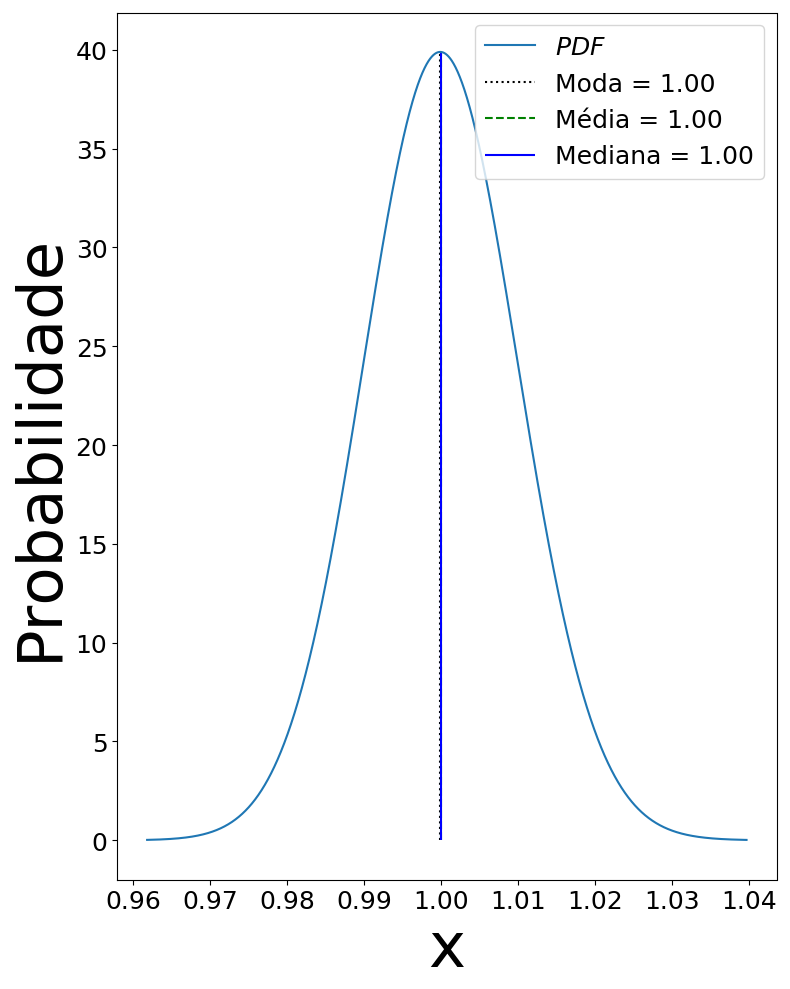
\includegraphics[width=\textwidth]{./figuras/log_sigma_001.png}
		\caption{}
		\label{fig:sig001}
	\end{subfigure}
	\hfill
	\begin{subfigure}[b]{0.3\textwidth}
		\centering 
		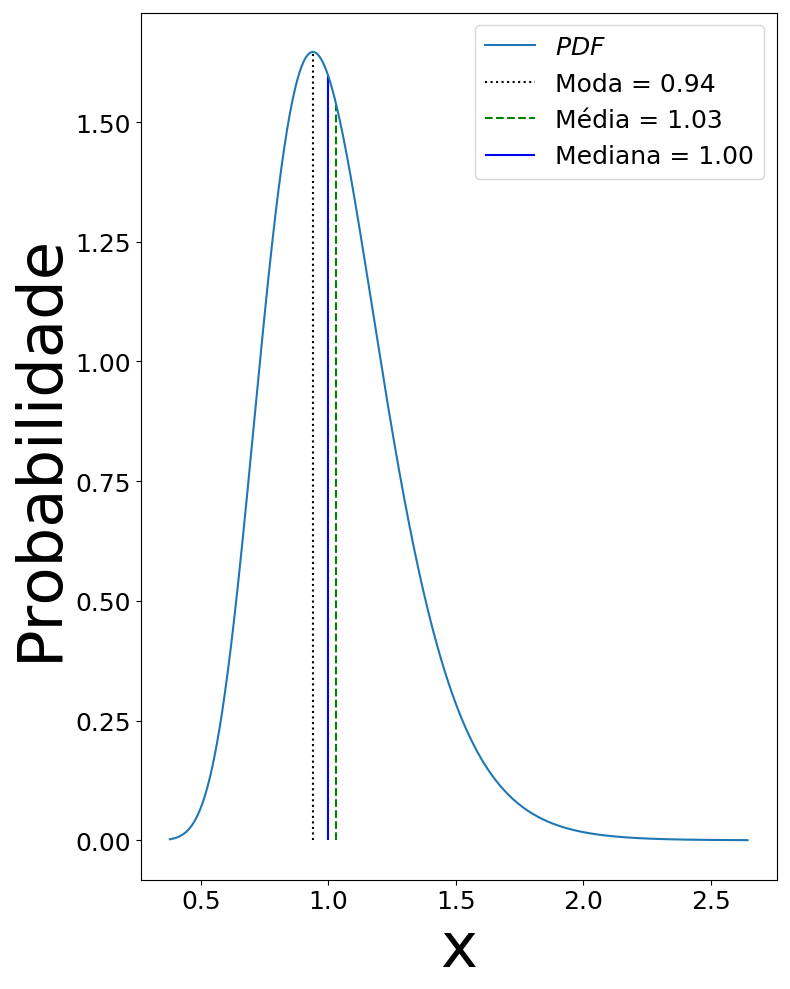
\includegraphics[width=\textwidth]{./figuras/log_sigma_025}
		\caption{}
		\label{fig:sig025}
	\end{subfigure}
	\hfill
	\begin{subfigure}[b]{0.3\textwidth}
		\centering 
		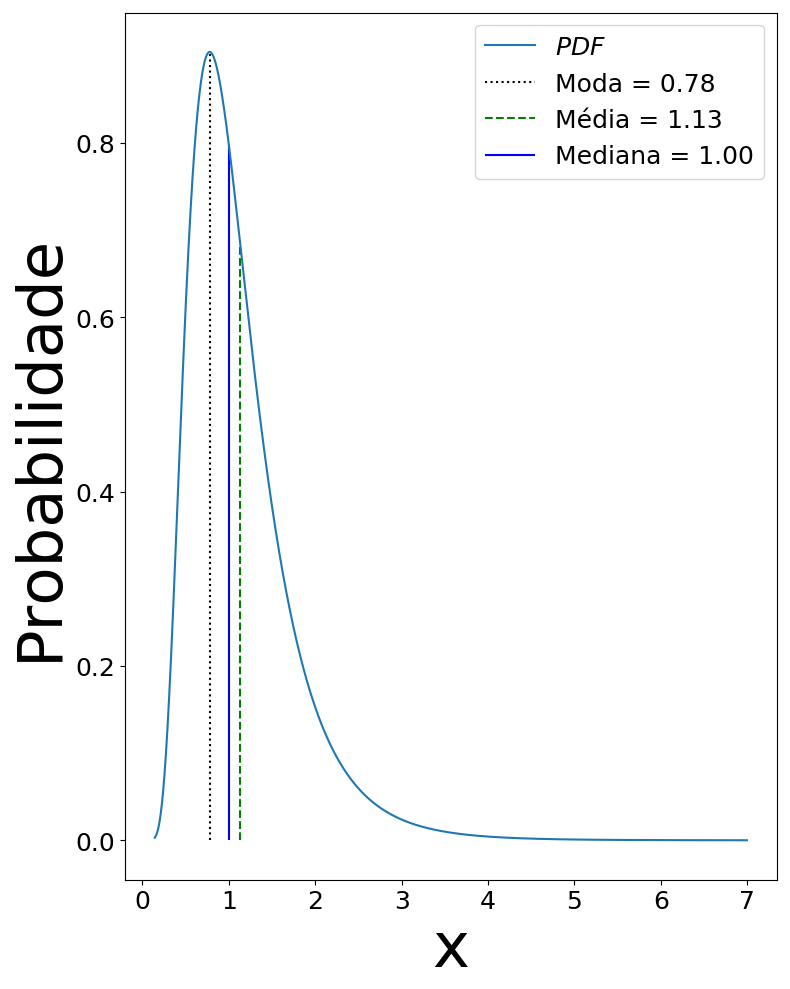
\includegraphics[width=\textwidth]{./figuras/log_sigma_05}
		\caption{}
		\label{fig:sig050}
	\end{subfigure}
	
	\begin{subfigure}[b]{0.3\textwidth}
		\centering 
		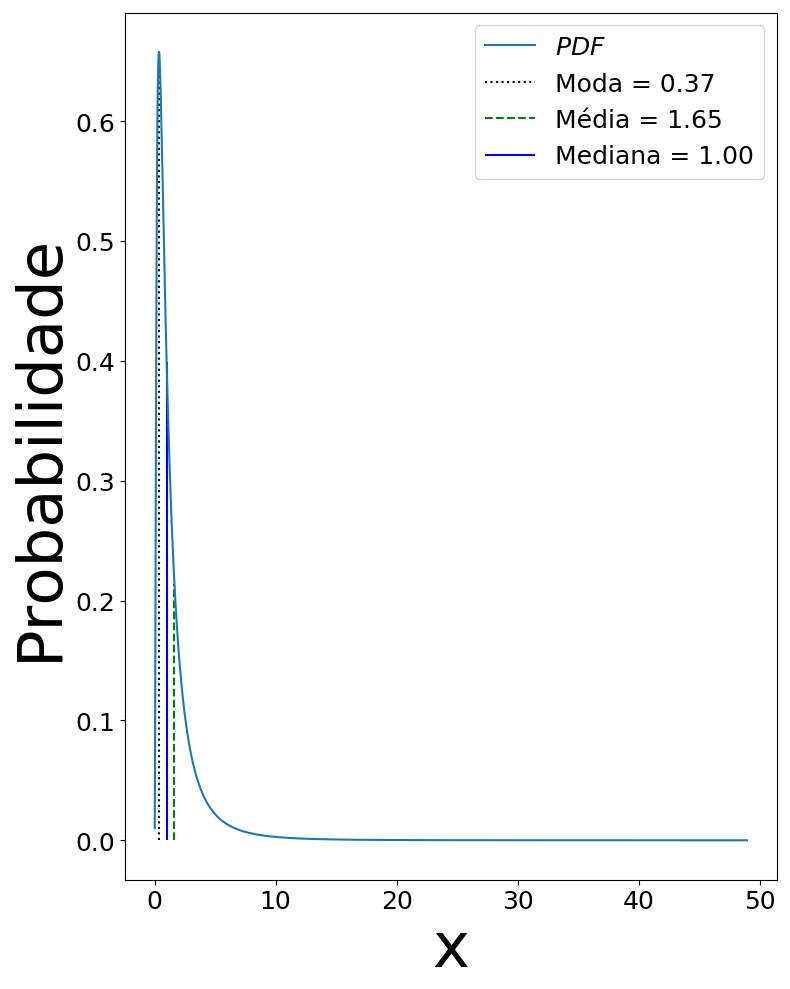
\includegraphics[width=\textwidth]{./figuras/log_sigma_1}
		\caption{}
		\label{fig:sig100}
	\end{subfigure}
	\hfill
	\begin{subfigure}[b]{0.3\textwidth}
		\centering 
		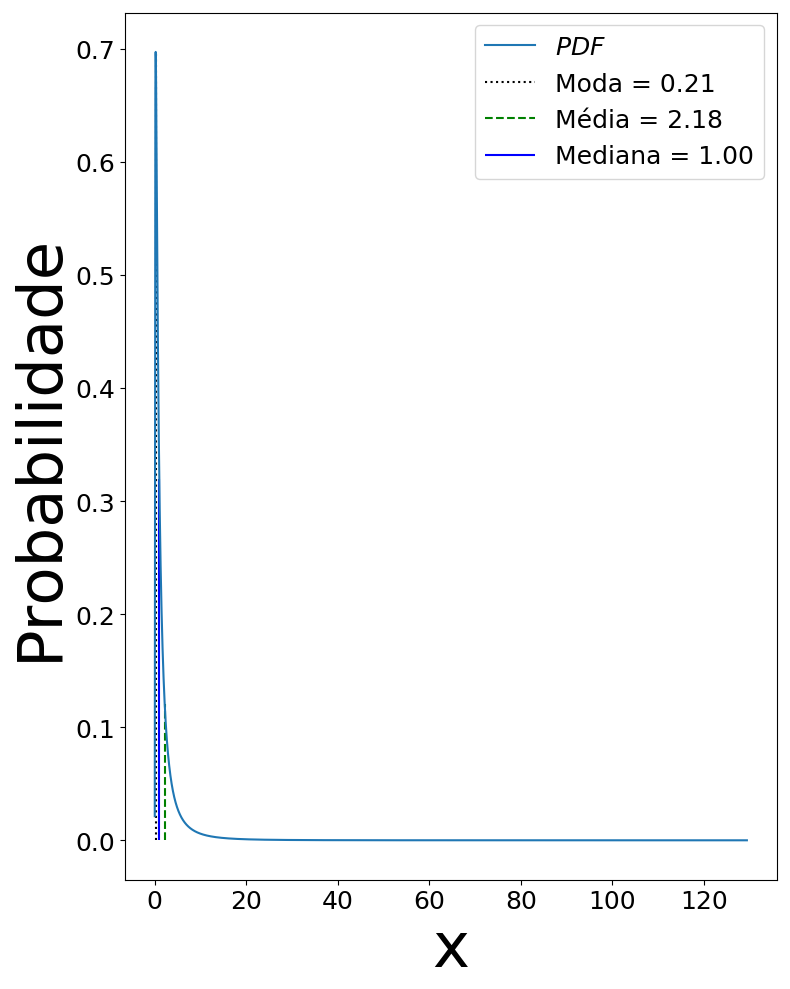
\includegraphics[width=\textwidth]{./figuras/log_sigma_125}
		\caption{}
		\label{fig:sig125}
	\end{subfigure}
	\hfill
	\begin{subfigure}[b]{0.3\textwidth}
		\centering 
		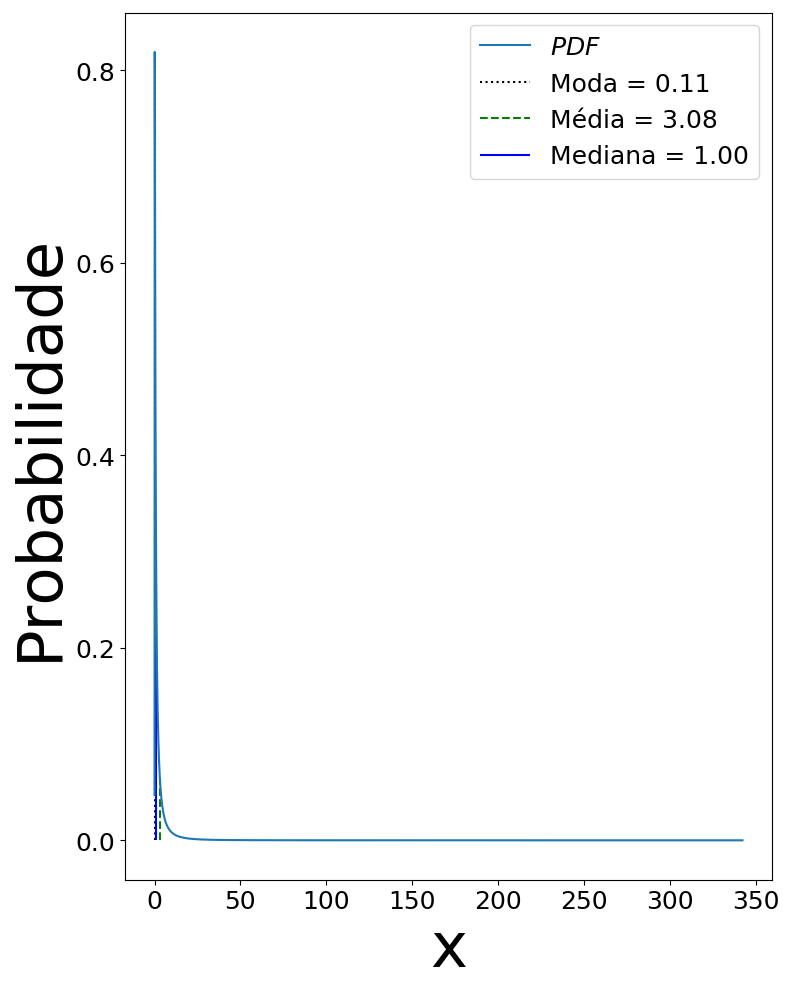
\includegraphics[width=\textwidth]{./figuras/log_sigma_15}
		\caption{}
		\label{fig:sig150}
	\end{subfigure}
	
	\caption{Ilustração das curvas Lognormais construidas com diferentes parâmetros: (a) possui $\sigma = 0.01$; (b) possui $\sigma = 0.25$; (c) possui $\sigma = 0.5$; (d) possui $\sigma = 1$; (e) possui $\sigma = 1.25$; e (f) possui $\sigma = 1.5$}
	\label{fig:Lognormal}
\end{figure}



\begin{figure}[H]
\centering
\begin{subfigure}[b]{0.27\textwidth}
	\centering 
	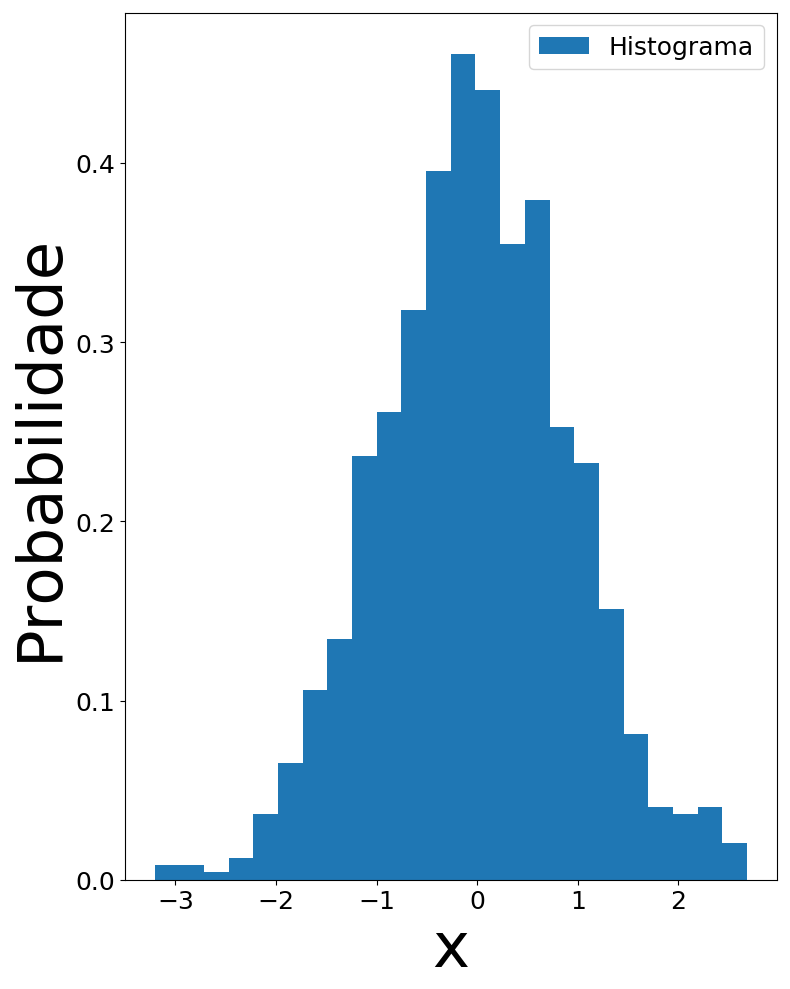
\includegraphics[width=\linewidth]{./figuras/datanormal_0}
	\caption{}
	\label{fig:randn}
\end{subfigure}
\hfill
\begin{subfigure}[b]{0.27\textwidth}
	\centering 
	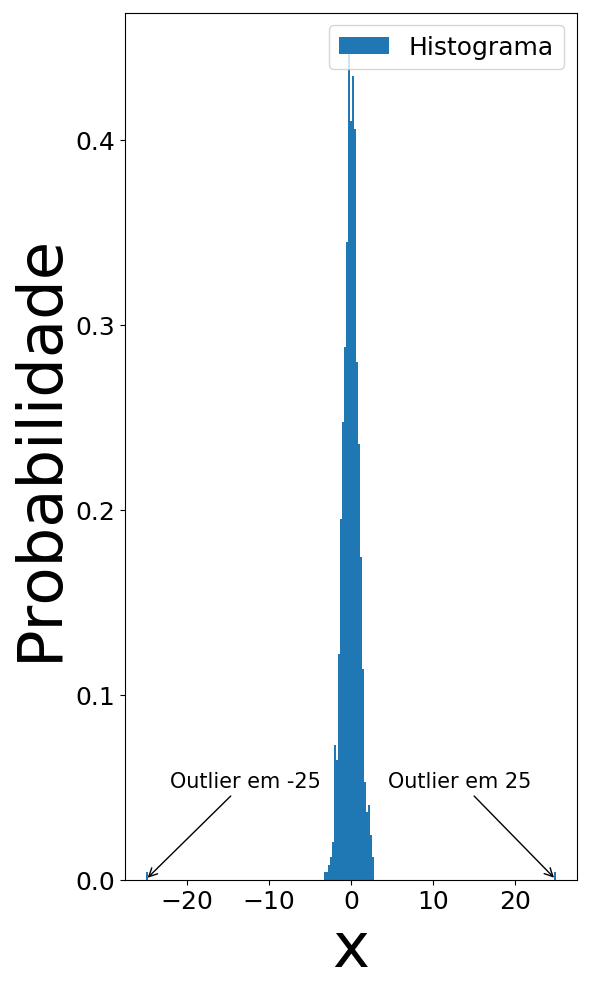
\includegraphics[width=\linewidth]{./figuras/datanormal_25}
	\caption{}
	\label{fig:randn_out}
\end{subfigure}
\hfill
\begin{subfigure}[b]{0.27\textwidth}
	\centering 
	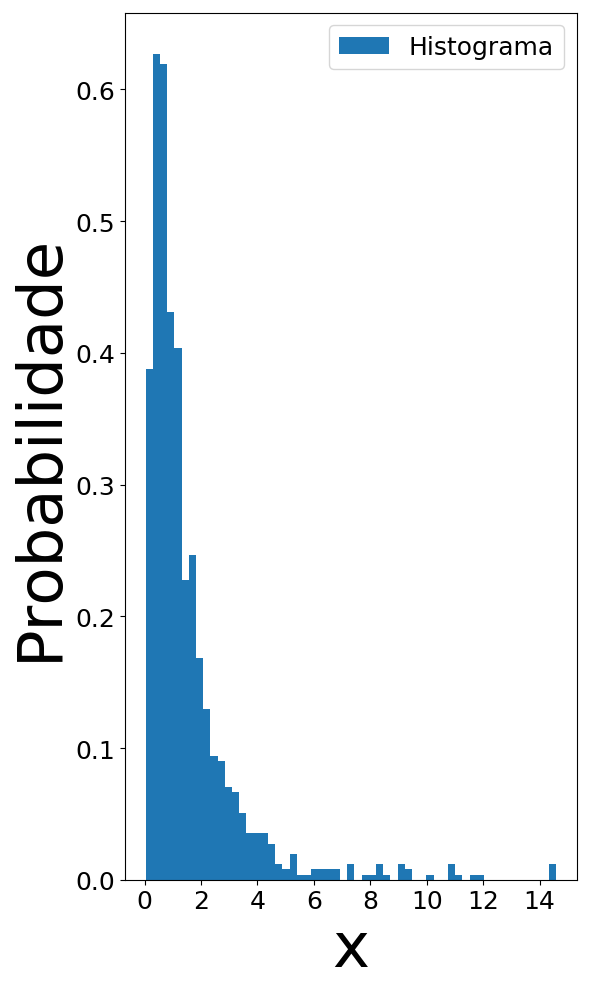
\includegraphics[width=\linewidth]{./figuras/datalognormal_0}
	\caption{}
	\label{fig:randlog}
\end{subfigure}

\caption{Histograma dos dados gerados sendo eles: (a) Gaussiana com $\mu = 0$ e $\sigma$ = 1; (b) Gaussiana com $\mu = 0$, $\sigma = 1$ e \textit{outlier} em $\pm 25$; (c) Lognormal com $\mu = 0$ e $\sigma = 1$.}
\label{fig:data}
\end{figure}

Os \textit{datasets} escolhidos possuem mil eventos, média $ \mu = 0 $ e são baseados na distribuição Gaussiana com desvio padrão $ \sigma = 1 $ sem \textit{outliers} ilustrado na Figura~\ref{fig:randn} e com \textit{outliers} em $ \pm 25 $ ilustrado  na Figura~\ref{fig:randn_out} e, por fim, baseado na distribuição Lognormal com desvio padrão $ \sigma = 1 $ ilustrado na Figura~\ref{fig:randlog}.



\section{Algoritmo}

O algoritmo para comparação e validação dos métodos de discretização de estimação construído nesse trabalho pode ser resumido pelo diagrama de blocos da Figura \ref{fig:08}, sendo testado de duas maneiras diversas: utilizando somente a função analítica e usando os dados gerados a partir das funções geradoras.

\begin{figure}[H]
	\begin{center}
	%	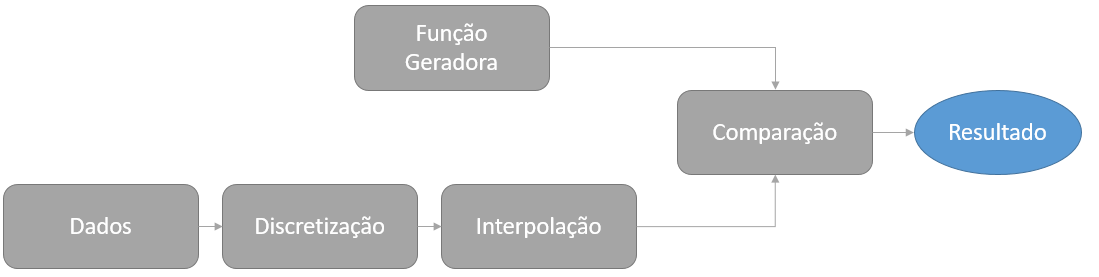
\includegraphics[width=0.5\linewidth]{./figuras/algoritmo1.png}
		\caption{Diagrama de blocos do algoritmo para validação dos métodos de discretização.}\label{fig:08}
	\end{center}
\end{figure}


\begin{description}
	\item[Função Analítica] Inicialmente uma função geradora é escolhida, sua discretização é feita utilizando os métodos apresentados, essa discretização é utilizada para calcular todos os pontos da curva original (utilizando interpolação) e por fim faz-se o cálculo da distância entre as duas curvas (analítica e discretizada) utilizando a métrica de distancia chamada L1, que é um caso particular da Equação \eqref{eq:4T06}.
	
	\begin{equation}\label{eq:4T06}
	{L_p} = {\left( {\int {{{\left| {f(x) - g(x)} \right|}^p}}\cdot dx } \right)^{{\raise0.7ex\hbox{$1$} \!\mathord{\left/
					{\vphantom {1 p}}\right.\kern-\nulldelimiterspace}
				\!\lower0.7ex\hbox{$p$}}}}
	\end{equation}
	
	Onde $p$ é o parâmetro a ser escolhido. No caso mais simples, $p=1$, a equação~\eqref{eq:4T06} se torna a equação~\eqref{eq:4T15}.
	
	\begin{equation}\label{eq:4T15}
	{L_1} = {\int {\left| {f(x) - g(x)} \right|} \cdot dx}
	\end{equation}
	
	A equação~\eqref{eq:4T15} é chamado de \ac{IAE} ou distância L1.
	
	\item[Dados gerados] Nesse caso, única diferença é que o calculo da discretização é feito usando como base a distribuição de eventos aleatórios geradas pela função geradora escolhida.
\end{description}

%\color{red} PAREI AQUI \color{black}

\section{Demostração dos métodos de discretização}

Com o intuito de validar os algoritmo e os métodos de discretização serão apresentados nessa seção o funcionamento desses métodos para a função gaussiana, função \textit{lognormal} e com dados gerados, representados pelas Figuras~\ref{fig:Gaussiana}, \ref{fig:Lognormal} e \ref{fig:data} respectivamente. E, com o objetivo de demostrar de forma mais clara o efeito desses métodos e sua dependência ao número de pontos de estimação escolhidos, os métodos serão avaliados variando o número de estimação para $ N = 15 $ e $ N = 25 $.

\subsection{Método \textit{Linspace}}

De acordo com o princípio de funcionamento do método de discretização \textit{Linspace} espera-se que este entregue resultados satisfatórios em distribuições com variações mais lentas, como mostrado nas Figuras~\ref{fig:lin_norm15}, \ref{fig:lin_norm25}, \ref{fig:lin_norm15_data} e \ref{fig:lin_norm25_data}. Já para conjunto de dados que apresenta variações mais rápidas ou \textit{outliers}, como mostrado nas Figuras~\ref{fig:lin_log15}, \ref{fig:lin_log25}, \ref{fig:lin_norm15_data_out} e \ref{fig:lin_norm25_data_out}, este método não alcança uma boa representação da PDF.


\begin{figure}[ht]
	\centering
	\begin{subfigure}[b]{0.45\textwidth}
		\centering 
		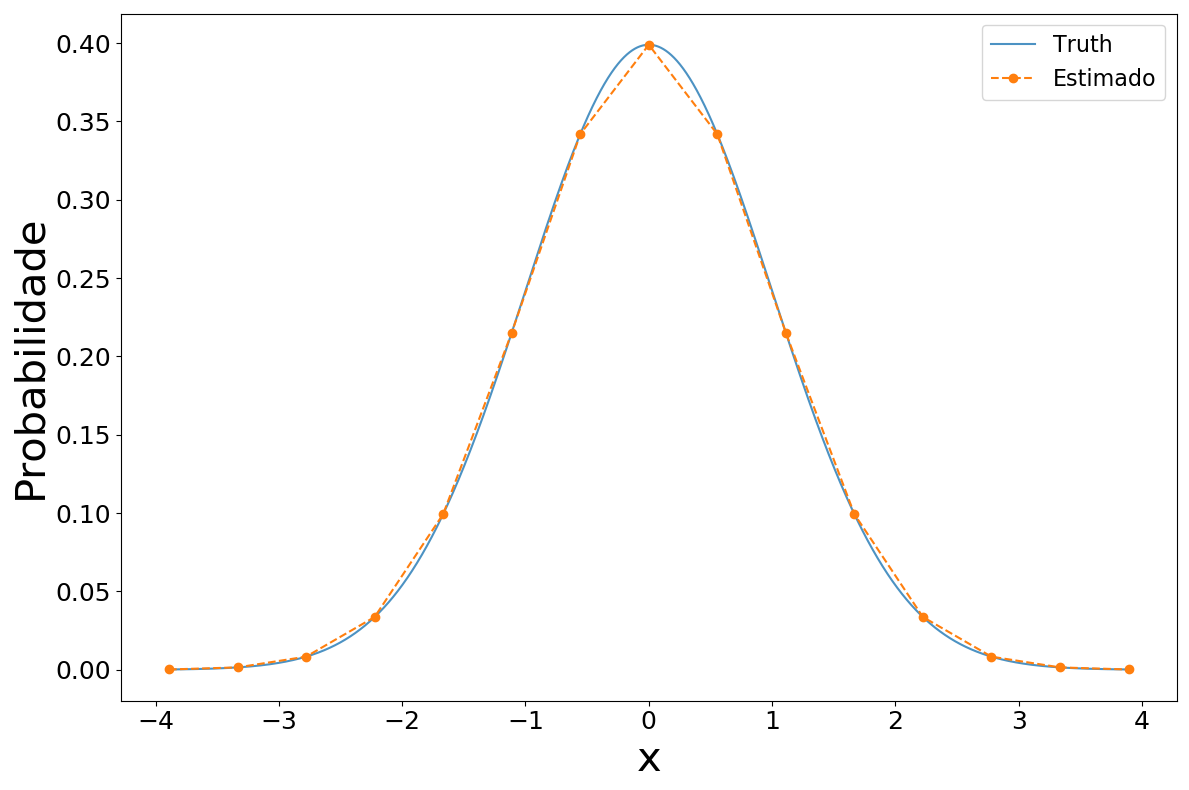
\includegraphics[width=\linewidth]{./figuras/Linspace_normal_15}
		\caption{}
		\label{fig:lin_norm15}
	\end{subfigure}
	\hfill
	\begin{subfigure}[b]{0.45\textwidth}
		\centering 
		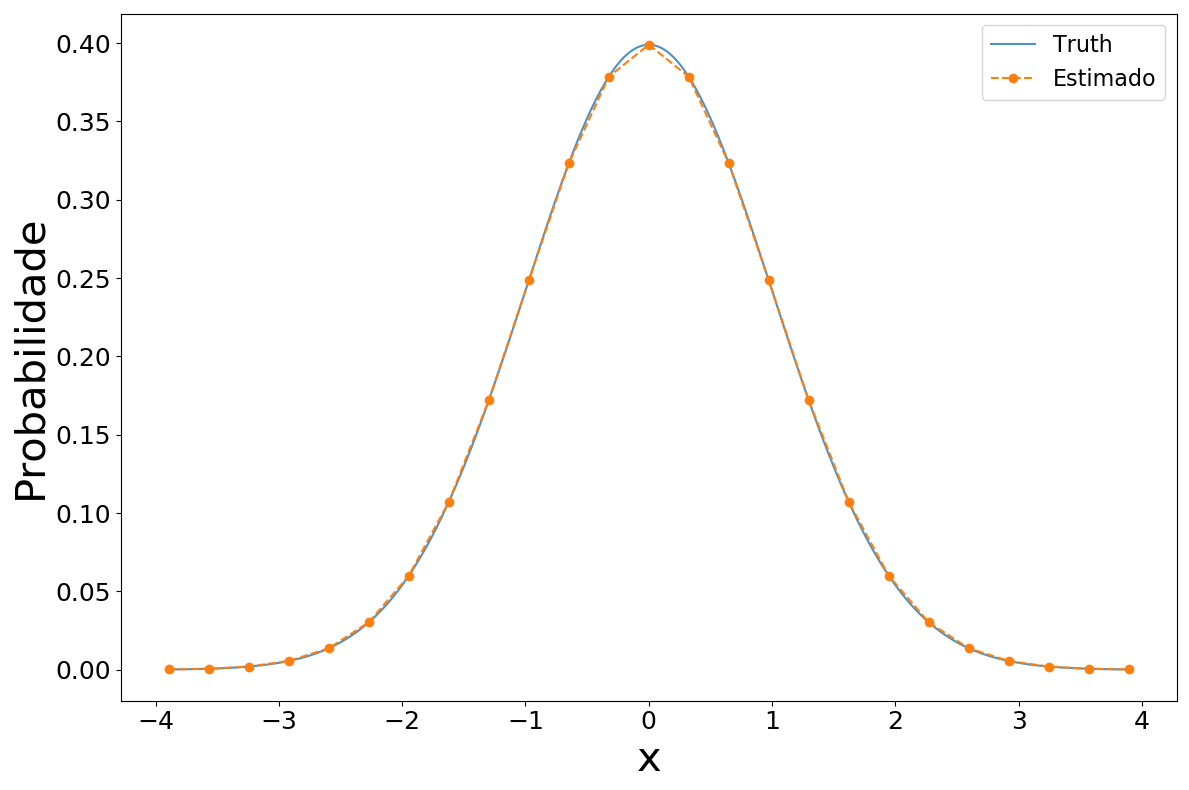
\includegraphics[width=\linewidth]{./figuras/Linspace_normal_25}
		\caption{}
		\label{fig:lin_norm25}
	\end{subfigure}
	\\
	\begin{subfigure}[b]{0.45\textwidth}
		\centering 
		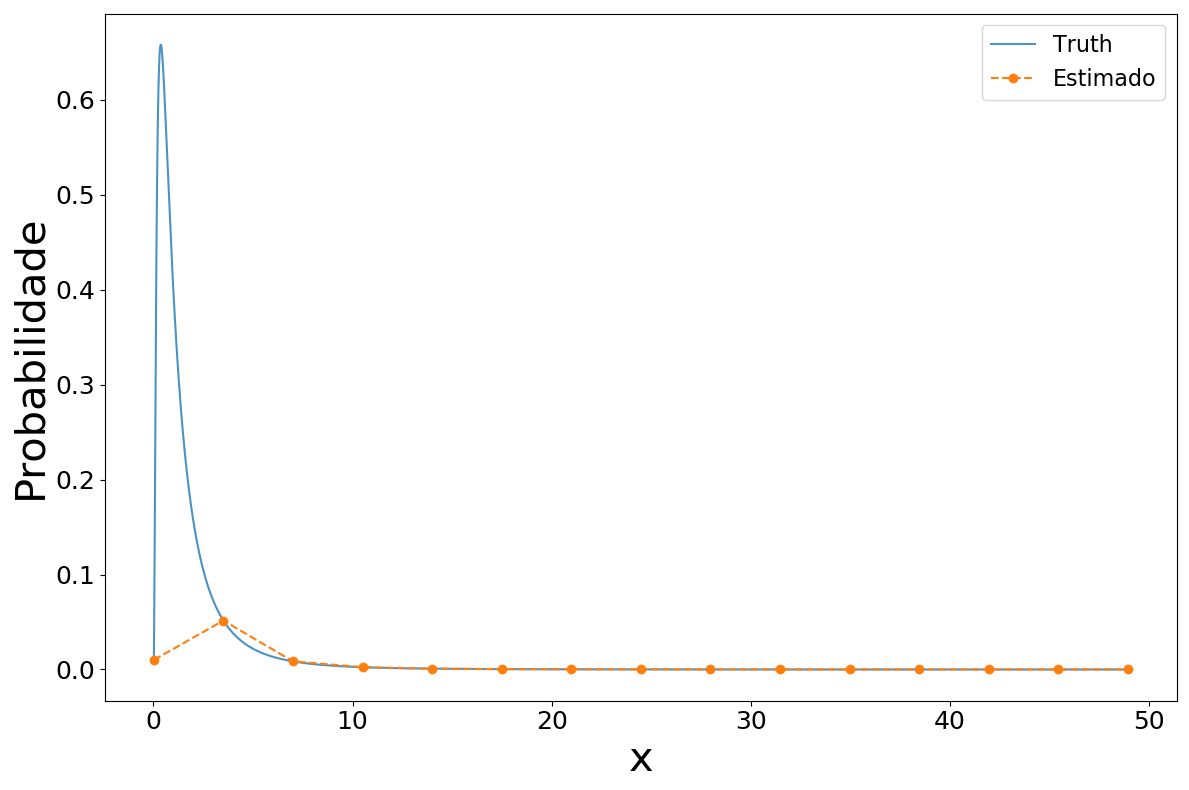
\includegraphics[width=\linewidth]{./figuras/Linspace_lognormal_15}
		\caption{}
		\label{fig:lin_log15}
	\end{subfigure}
	\hfill
	\begin{subfigure}[b]{0.45\textwidth}
		\centering 
		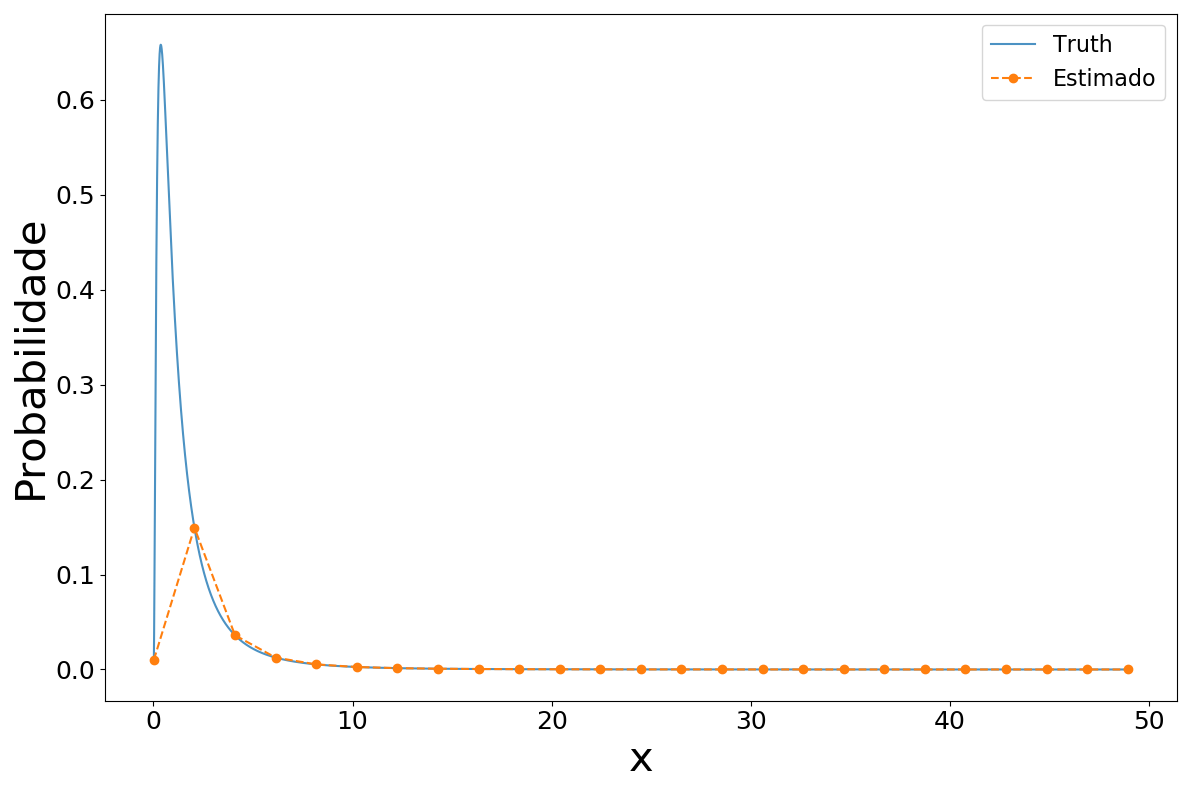
\includegraphics[width=\linewidth]{./figuras/Linspace_lognormal_25}
		\caption{}
		\label{fig:lin_log25}
	\end{subfigure}
	
	\caption{Discretização utilizando o método de \textit{Linspace}: (a) N(0,1) com $N = 15$, (b) N(0,1) com $N = 25$, (c) L(0,1) com $N = 15$ e (d) L(0,1) com $N = 25$.}
	\label{fig:normlin}
\end{figure}


\begin{figure}[H]
	\centering\begin{subfigure}[b]{0.45\textwidth}
		\centering 
		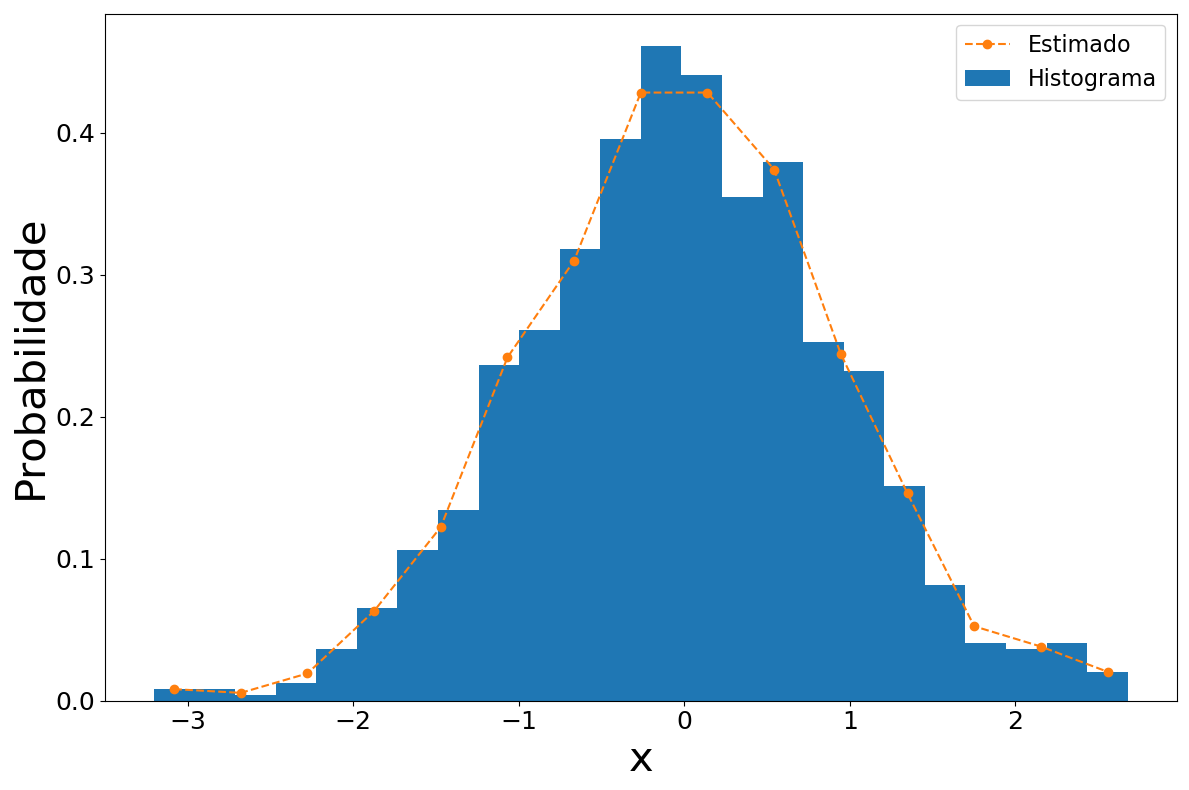
\includegraphics[width=\linewidth]{./figuras/Linspace_normal_15_1000_0}
		\caption{}
		\label{fig:lin_norm15_data}
	\end{subfigure}
	\hfill
	\begin{subfigure}[b]{0.45\textwidth}
		\centering 
		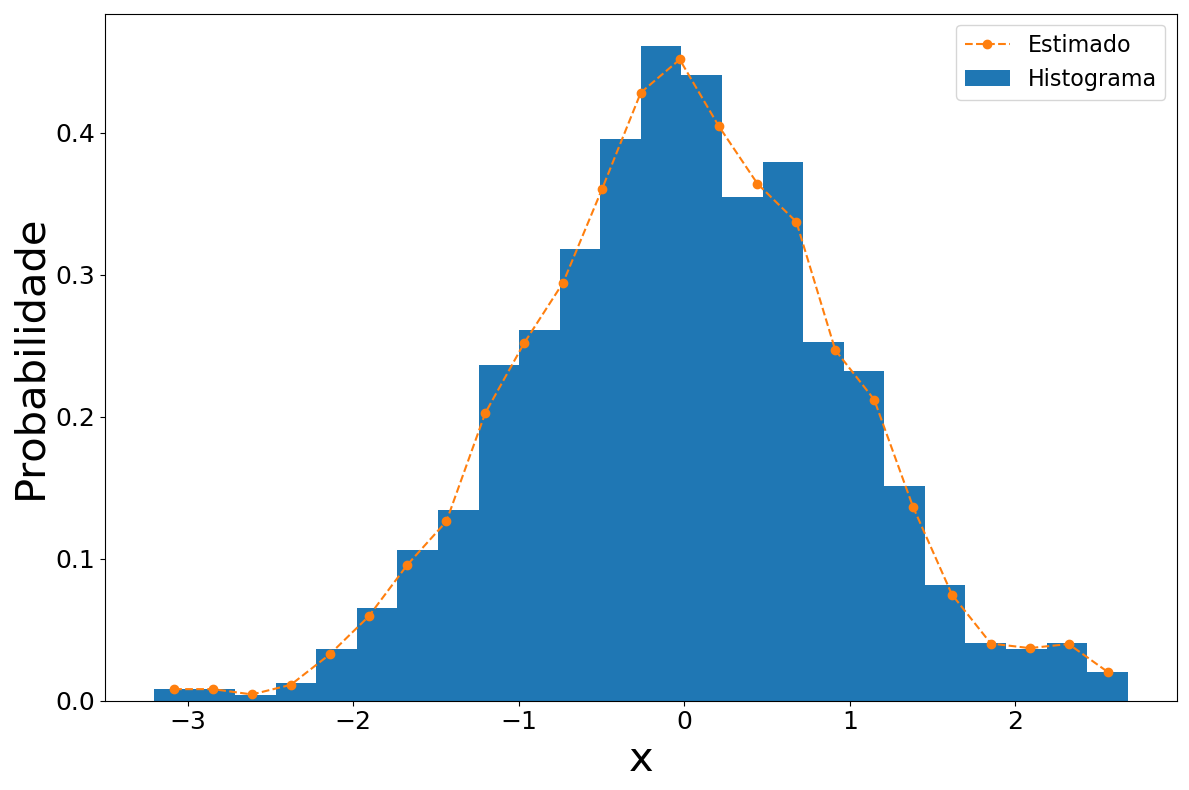
\includegraphics[width=\linewidth]{./figuras/Linspace_normal_25_1000_0}
		\caption{}
		\label{fig:lin_norm25_data}
	\end{subfigure}
	\\
	\begin{subfigure}[b]{0.45\textwidth}
		\centering 
		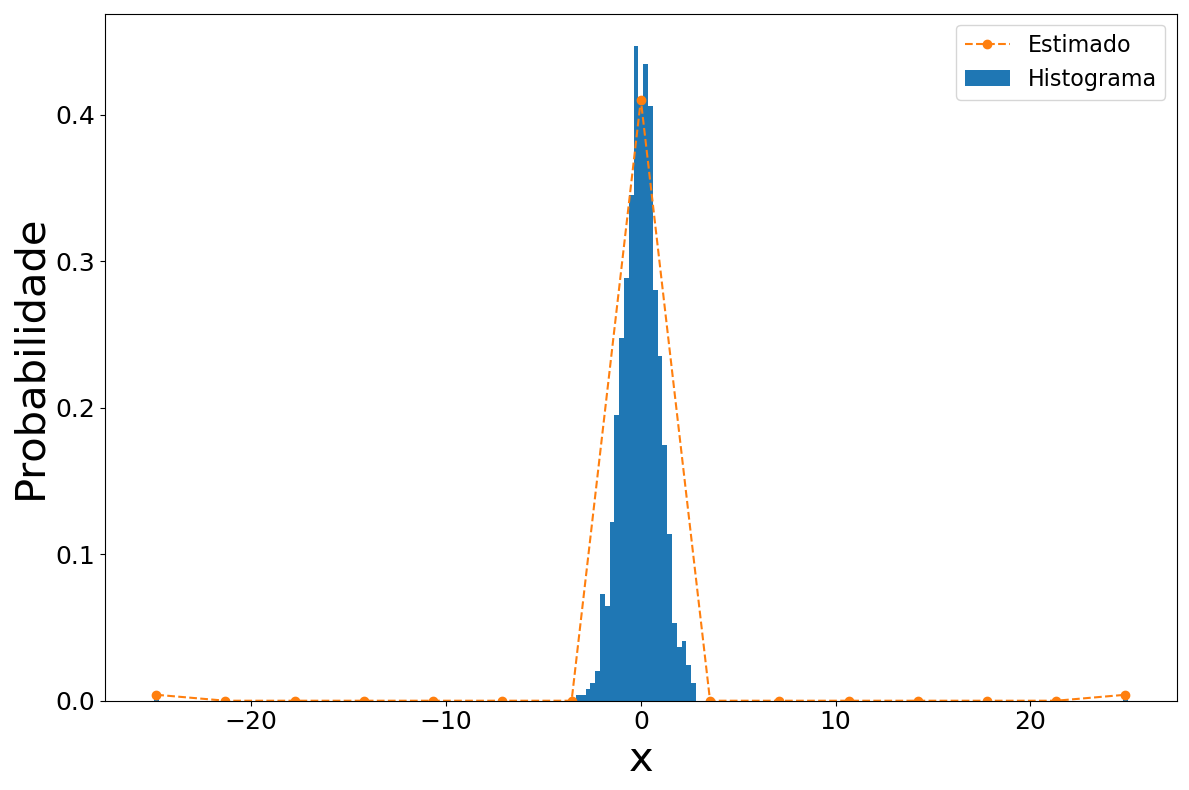
\includegraphics[width=\linewidth]{./figuras/Linspace_normal_15_1000_25}
		\caption{}
		\label{fig:lin_norm15_data_out}
	\end{subfigure}
	\hfill
	\begin{subfigure}[b]{0.45\textwidth}
		\centering 
		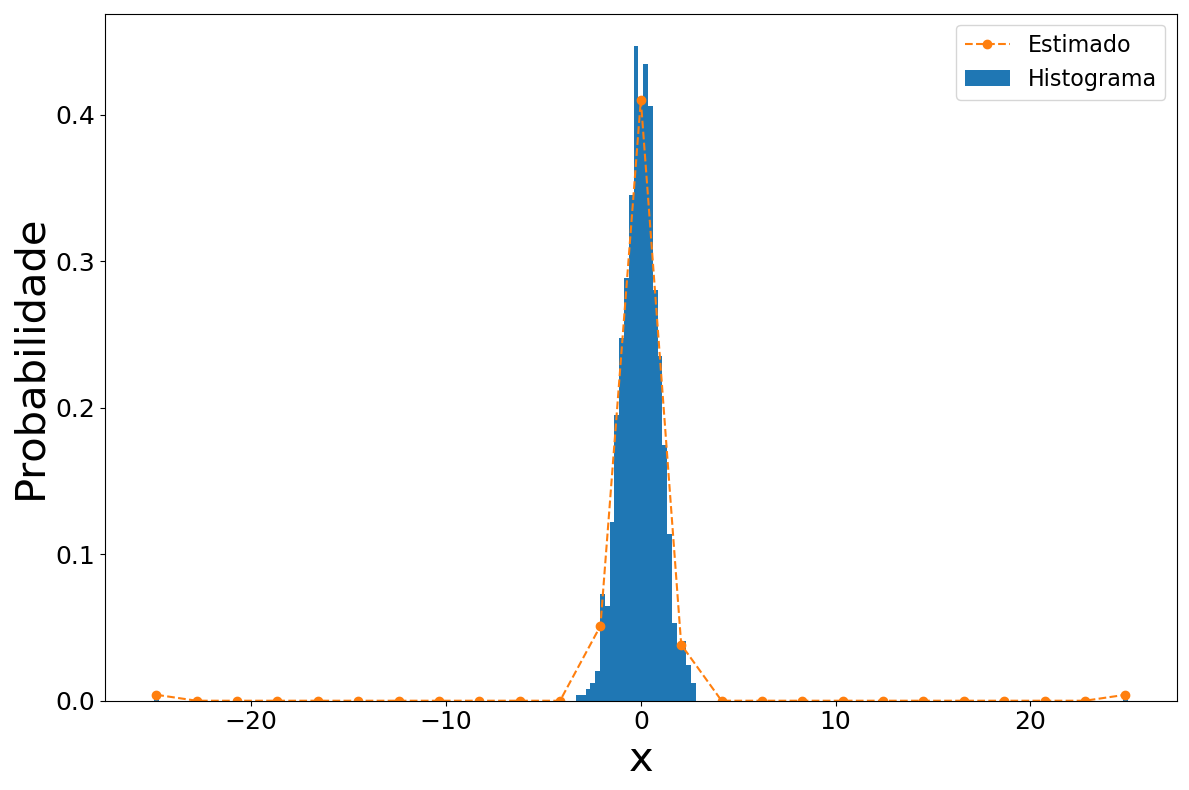
\includegraphics[width=\linewidth]{./figuras/Linspace_normal_25_1000_25}
		\caption{}
		\label{fig:lin_norm25_data_out}
	\end{subfigure}
	\\
	\begin{subfigure}[b]{0.45\textwidth}
		\centering 
		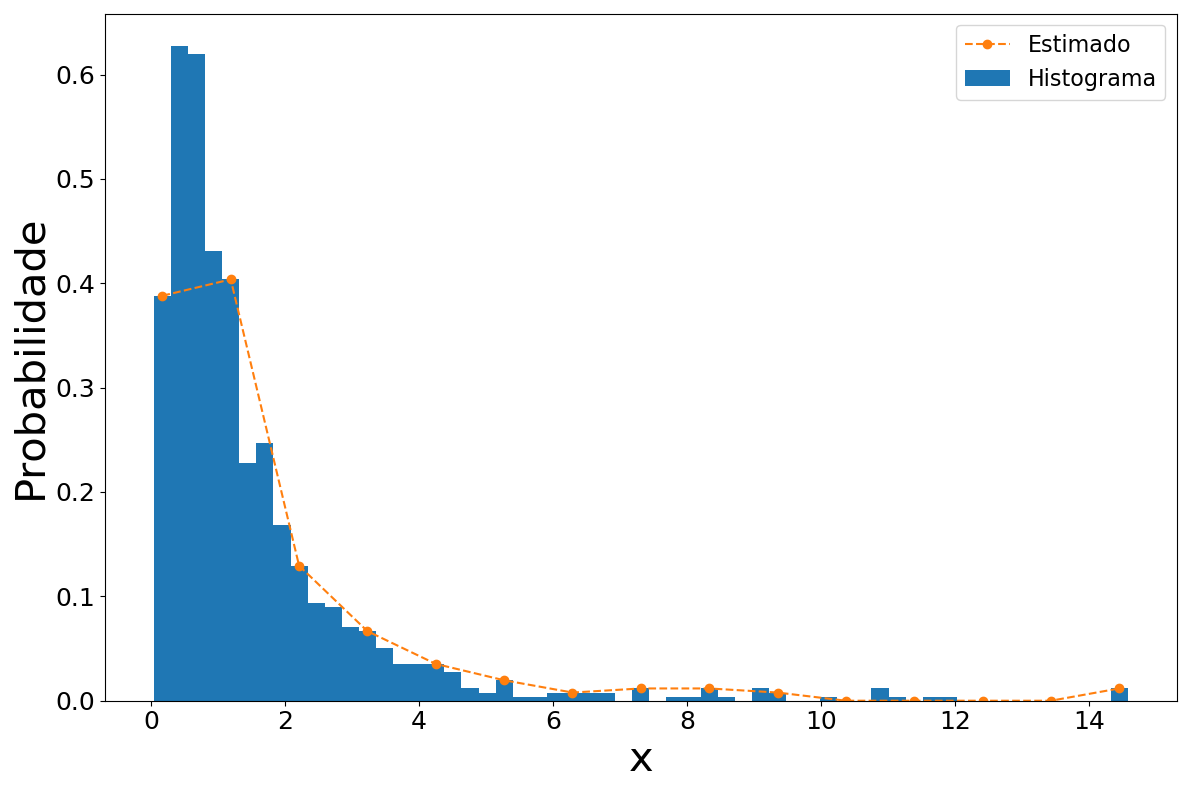
\includegraphics[width=\linewidth]{./figuras/Linspace_lognormal_15_1000}
		\caption{}
		\label{fig:lin_lognorm15_data}
	\end{subfigure}
	\hfill
	\begin{subfigure}[b]{0.45\textwidth}
		\centering 
		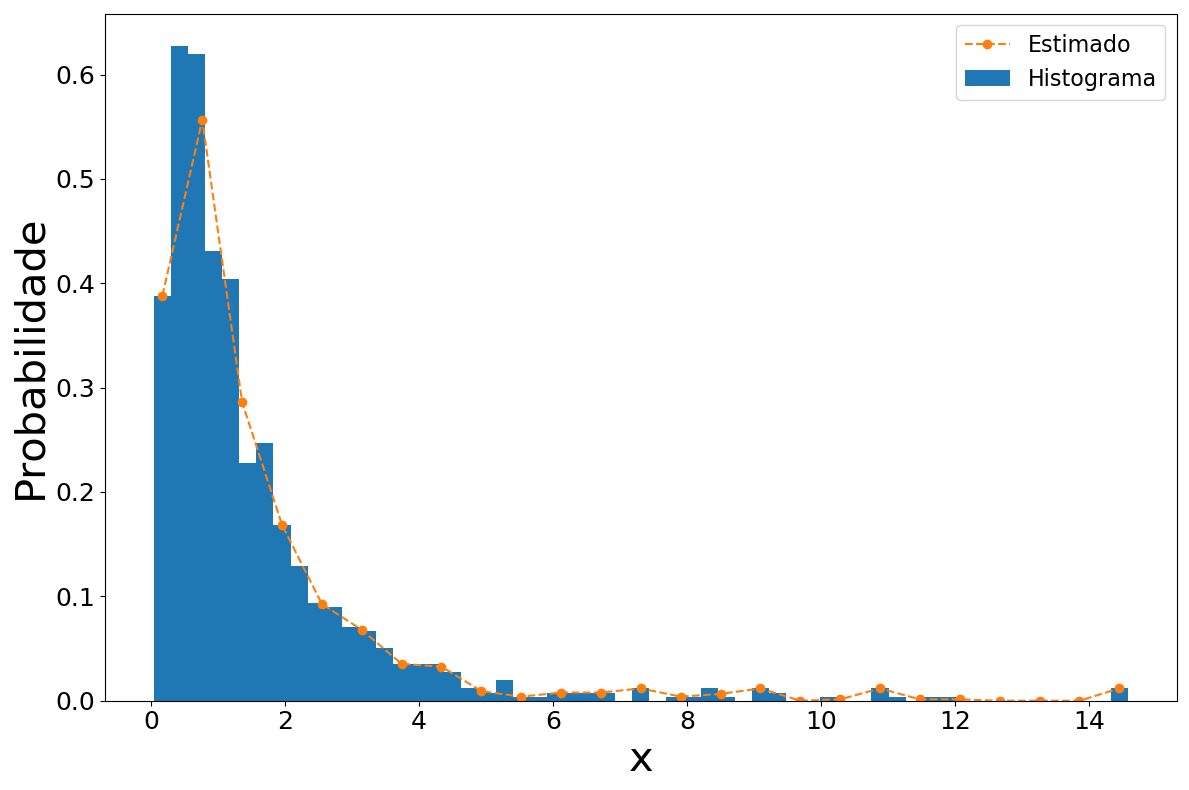
\includegraphics[width=\linewidth]{./figuras/Linspace_lognormal_25_1000}
		\caption{}
		\label{fig:lin_lognorm25_data}
	\end{subfigure}
	\caption{Discretização com os dados gerados utilizando o método de \textit{Linspace}: (a) randN(0,1) com $N = 15$, (b) randN(0,1) com $N = 25$, (c) randN(0,1) com $N = 15$ e \textit{outlier} em $\pm 25$, (d) randN(0,1) com $N = 25$ e \textit{outlier} em $\pm 25$, (e) randL(0,1) com $ N = 15 $ e (f) randL(0,1) com $ N = 25 $.}
	\label{fig:lin_data}
\end{figure}

Entretanto, pode-se perceber que com o aumento do número de pontos de estimação ($N = 15$ para $N = 25$) o desempenho deste método apresenta uma melhora significativa, portanto, fica claro que é possível alcançar uma boa performance com o método de \textit{Linspace}. Mas, há de se comentar que o aumento do número de pontos de estimação é um fator decisivo no custo computacional desses algoritmos, além disso, aumenta a quantidade de informação a ser armazenada ou transmitida e, apesar da distribuição randL(0,1) ser baseada na L(0,1), está apresenta uma melhor discretização devido ao fato da sua extensão no eixo $ x $ ser menor. As distribuições L(0,0.01), L(0,0.25) e L(0,0.5) possuem um comportamento semelhante à N(0,1), enquanto as distribuições L(0,1.25) e L(0,1.5) semelhantes à L(0,1) como pode ser visto no Apêndice~\ref{cap:anexoLin}

\subsection{Método \textit{CDFm}}

Pelo método \ac{CDFm} é esperado um acumulo maior de pontos nas regiões em que a probabilidade é maior, como é ilustrado nas Figuras~\ref{fig:cdfnorm} e \ref{fig:cdf_data}, porem, é possível perceber que quanto mais rápida é a variação, melhor a sua discretização como é notado comparando as Figuras~\ref{fig:cdfnorm15} e \ref{fig:cdf_log15} e que \textit{outliers} não impactam tanto a discretização, mostrado nas Figuras~\ref{fig:cdf_norm15_data_out} e \ref{fig:cdf_lognorm25_data}. Esse mesmo padrão se repete tando com os dados gerados mostrado na Figura~\ref{fig:cdf_data} quanto nas outras distribuições Lognormais, mostradas no Apêndice~\ref{cap:anexoCDFm}.

\begin{figure}[H]
	\centering
	\begin{subfigure}[b]{0.45\textwidth}
		\centering 
		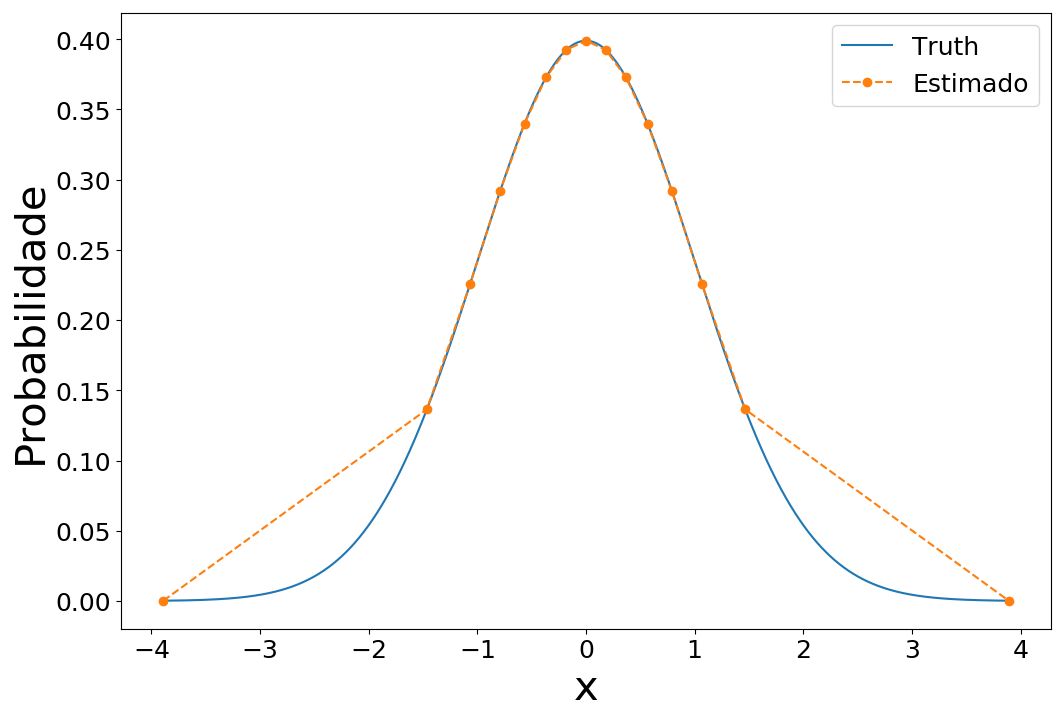
\includegraphics[width=\linewidth]{./figuras/CDFm_normal_15}
		\caption{}
		\label{fig:cdfnorm15}
	\end{subfigure}
	\hfill
	\begin{subfigure}[b]{0.45\textwidth}
		\centering 
		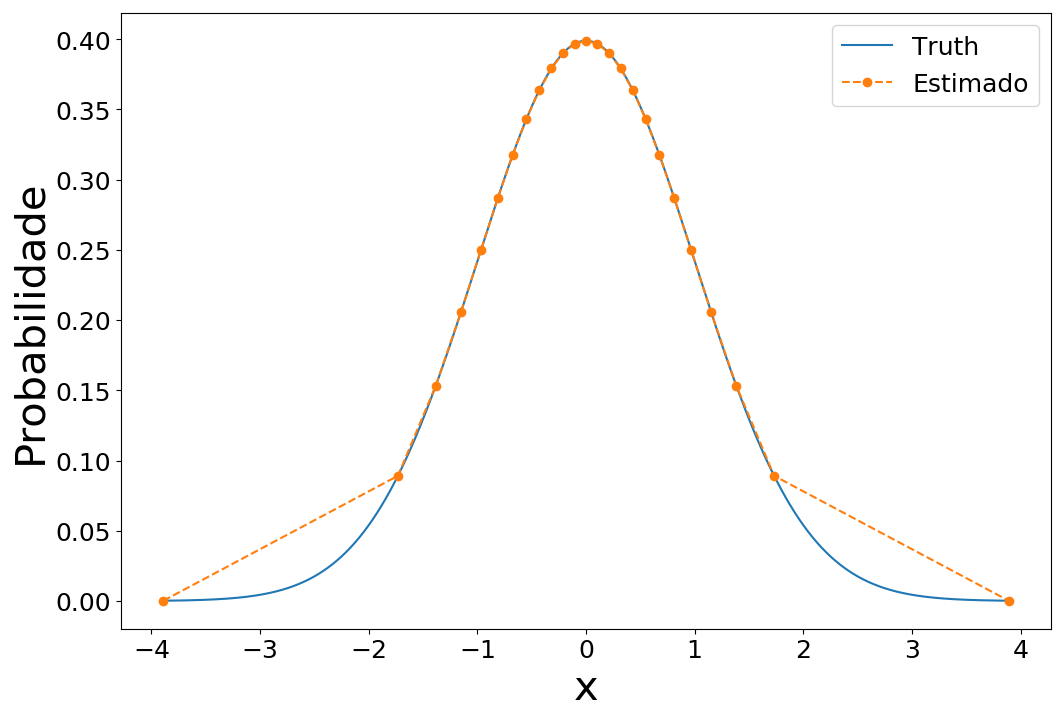
\includegraphics[width=\linewidth]{./figuras/CDFm_normal_25}
		\caption{}
		\label{fig:cdfnorm25}
	\end{subfigure}
	
	
	\begin{subfigure}[b]{0.45\textwidth}
		\centering 
		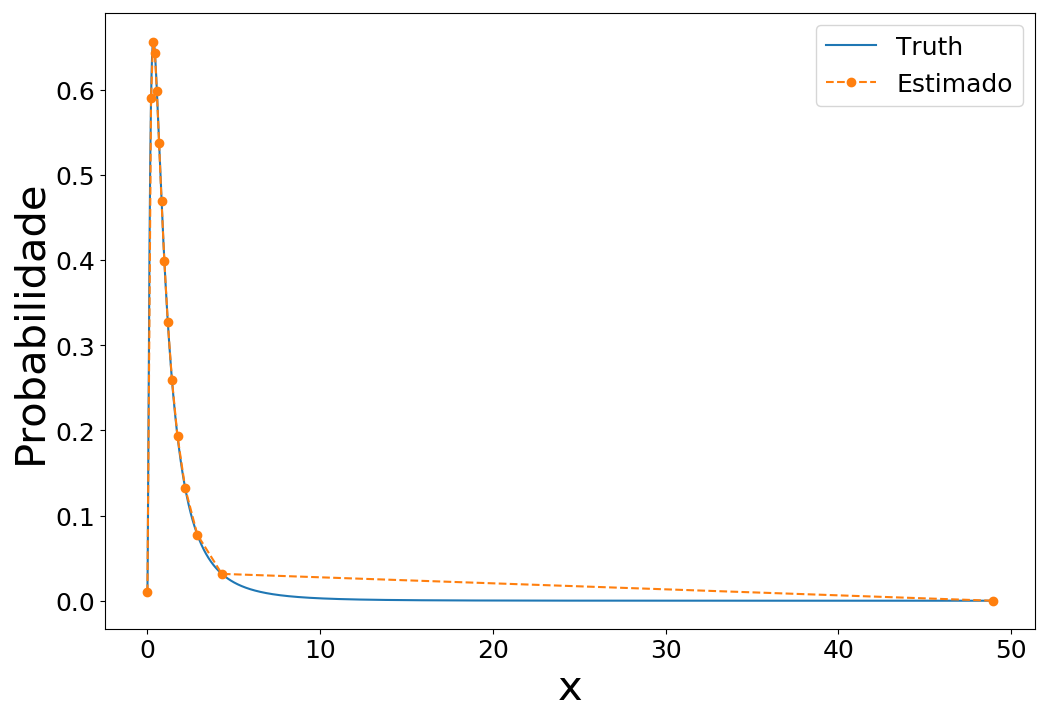
\includegraphics[width=\linewidth]{./figuras/CDFm_lognormal_15}
		\caption{}
		\label{fig:cdf_log15}
	\end{subfigure}
	\hfill
	\begin{subfigure}[b]{0.45\textwidth}
		\centering 
		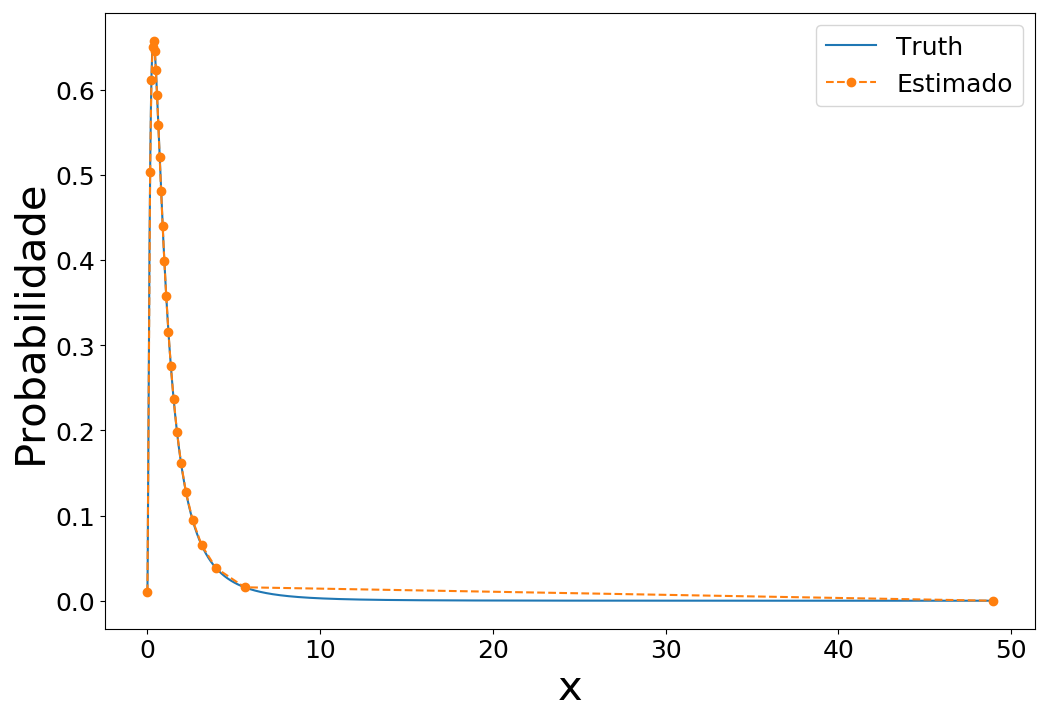
\includegraphics[width=\linewidth]{./figuras/CDFm_lognormal_25}
		\caption{}
		\label{fig:cdf_log25}
	\end{subfigure}
	
	\caption{Discretização utilizando o método de \textit{CDFm}: (a) N(0,1) com $N = 15$, (b) N(0,1) com $N = 25$, (c) L(0,1) com $N = 15$ e (d) L(0,1) com $N = 25$.}
	\label{fig:cdfnorm}
\end{figure}

\begin{figure}[H]
	\centering\begin{subfigure}[b]{0.45\textwidth}
		\centering 
		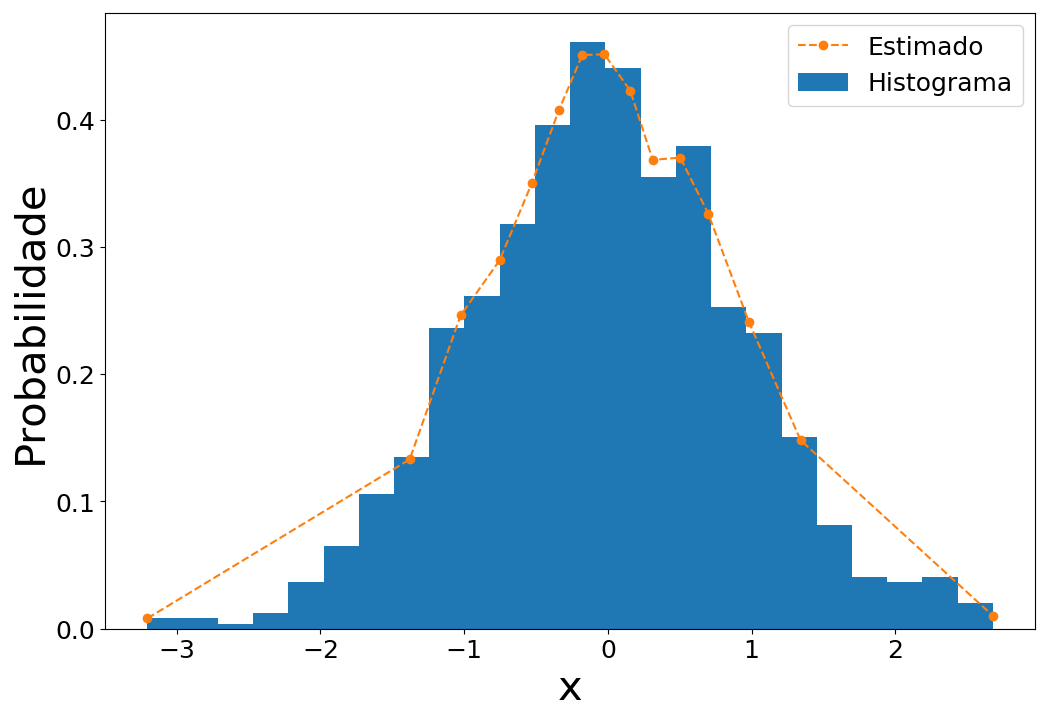
\includegraphics[width=\linewidth]{./figuras/CDFm_normal_15_1000_0}
		\caption{}
		\label{fig:cdf_norm15_data}
	\end{subfigure}
	\hfill
	\begin{subfigure}[b]{0.45\textwidth}
		\centering 
		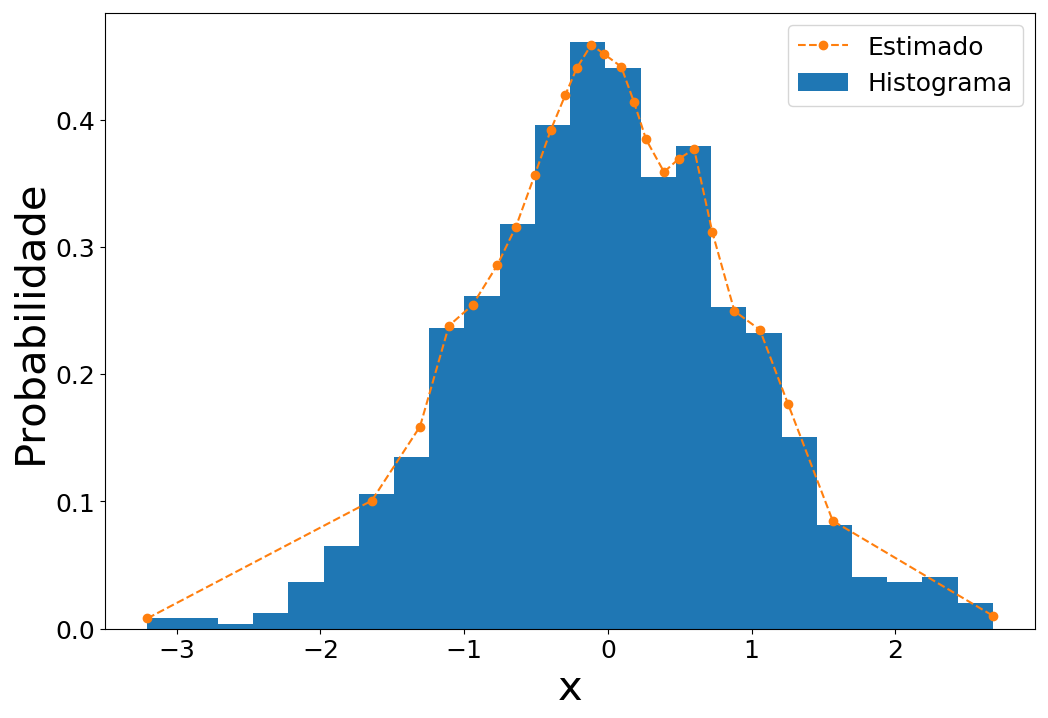
\includegraphics[width=\linewidth]{./figuras/CDFm_normal_25_1000_0}
		\caption{}
		\label{fig:cdf_norm25_data}
	\end{subfigure}
	\\
	\begin{subfigure}[b]{0.45\textwidth}
		\centering 
		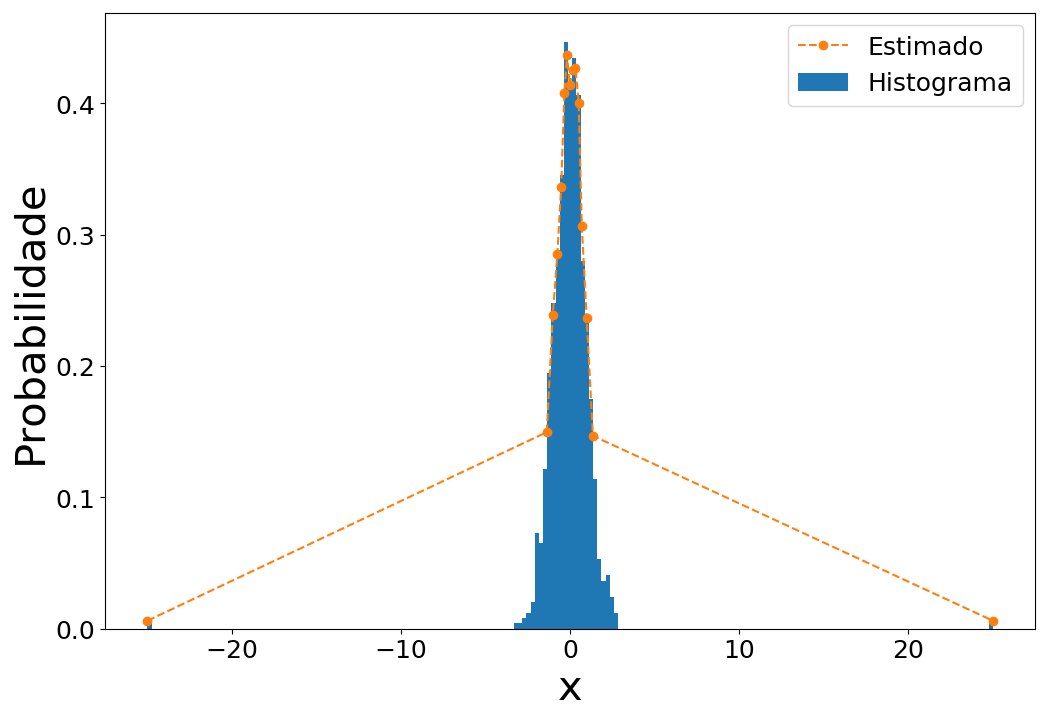
\includegraphics[width=\linewidth]{./figuras/CDFm_normal_15_1000_25}
		\caption{}
		\label{fig:cdf_norm15_data_out}
	\end{subfigure}
	\hfill
	\begin{subfigure}[b]{0.45\textwidth}
		\centering 
		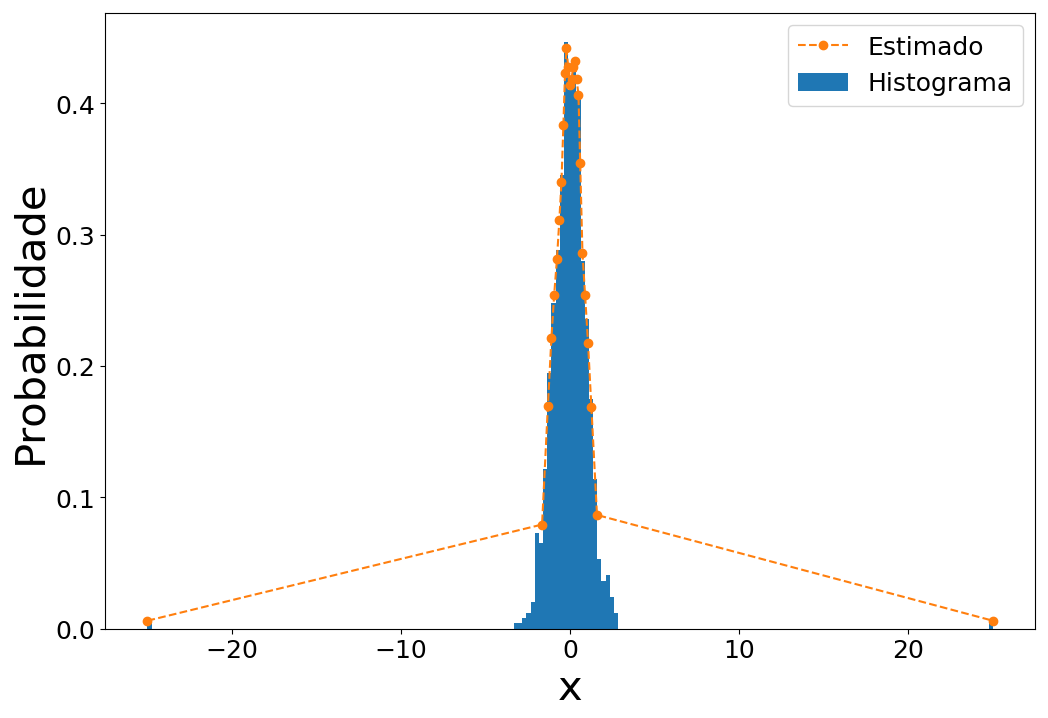
\includegraphics[width=\linewidth]{./figuras/CDFm_normal_25_1000_25}
		\caption{}
		\label{fig:cdf_norm25_data_out}
	\end{subfigure}
	\\
	\begin{subfigure}[b]{0.45\textwidth}
		\centering 
		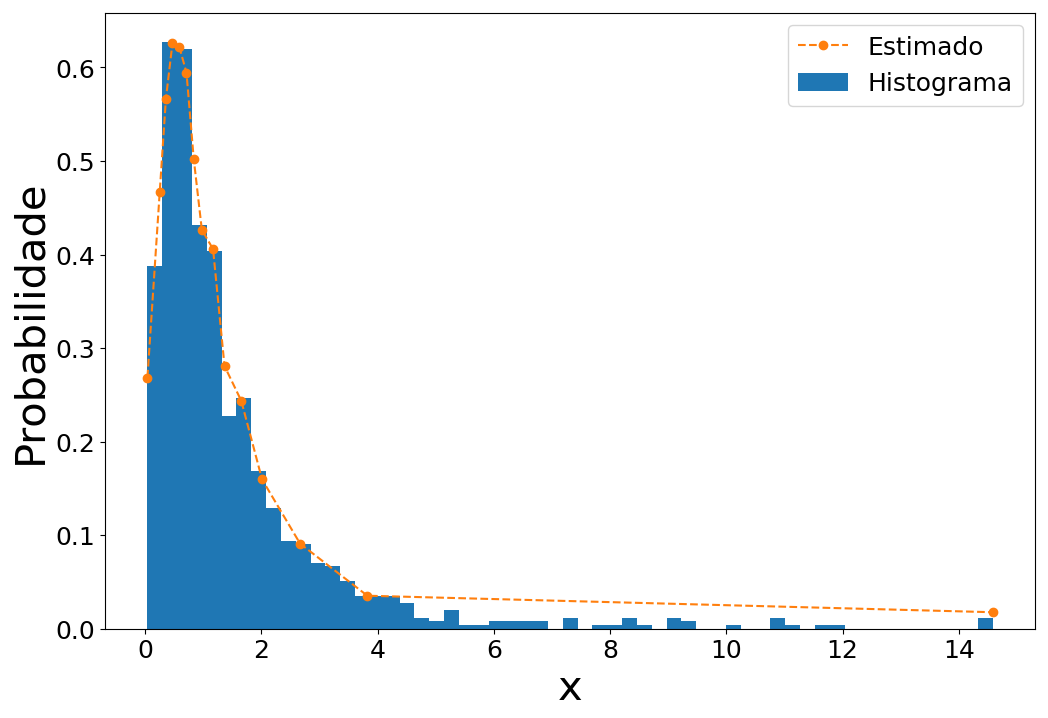
\includegraphics[width=\linewidth]{./figuras/CDFm_lognormal_15_1000_0}
		\caption{}
		\label{fig:cdf_lognorm15_data}
	\end{subfigure}
	\hfill
	\begin{subfigure}[b]{0.45\textwidth}
		\centering 
		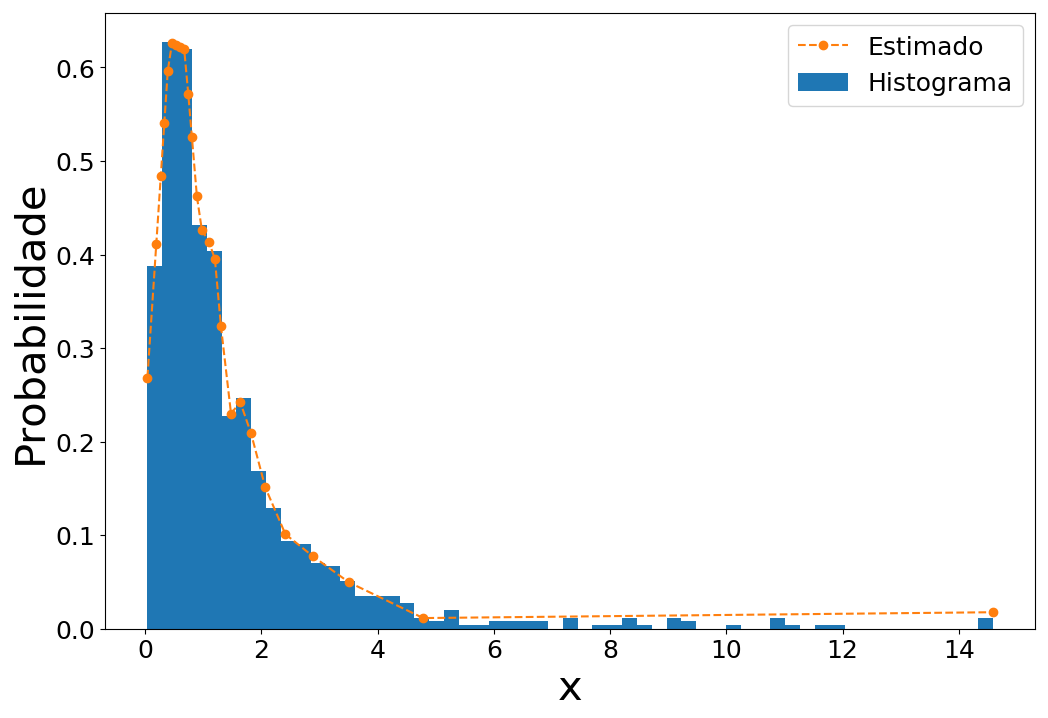
\includegraphics[width=\linewidth]{./figuras/CDFm_lognormal_25_1000_0}
		\caption{}
		\label{fig:cdf_lognorm25_data}
	\end{subfigure}
	\caption{Discretização com os dados gerados utilizando o método \ac{CDFm}: (a) randN(0,1) com $N = 15$, (b) randN(0,1) com $N = 25$, (c) randN(0,1) com $N = 15$ e \textit{outlier} em $\pm 25$, (d) randN(0,1) com $N = 25$ e \textit{outlier} em $\pm 25$, (e) randL(0,1) com $ N = 15 $ e (f) randL(0,1) com $ N = 25 $.}
	\label{fig:cdf_data}
\end{figure}

Este método, se comparado ao \textit{Linspace} apresenta um erro muito menor nas regiões de alta probabilidade, em contrapartida, ele não deve ser indicado quando o objeto de estudo é a análise de eventos em regiões de baixa probabilidade, pois o mesmo teria que ter um número de pontos superior para o estudo dessas regiões.
%Vemos que a região de alta probabilidade é representada com um menor erro do que no método \textit{Linspace} mas, em contrapartida, a região de baixa probabilidade necessitaria de um número muito maior de pontos para possuir o mesmo erro do método anterior.

\subsection{Método \textit{PDFm}}

Como este método divide o eixo $ y $ de maneira uniforme, ele tende a penalizar menos as regiões de baixa probabilidade e que sejam simétricas se comparado com o método \ac{CDFm} como pode ser visto nas Figuras~\ref{fig:pdfnorm15}, \ref{fig:pdfnorm25}, \ref{fig:pdfm_norm15_data}, \ref{fig:pdfm_norm25_data}, \ref{fig:pdfm_norm15_data_out} e \ref{fig:pdfm_norm25_data_out}, já para o caso destas distribuições não serem simétricas, como mostra as Figuras~\ref{fig:pdflognorm15}, \ref{fig:pdflognorm15}, \ref{fig:pdfm_lognorm15_data} e \ref{fig:pdfm_lognorm25_data} a região de baixa probabilidade é mais afetada que o método anterior. Este padrão se repete para desvios padrões diferentes da distribuição Lognormal, que pode ser observado no Apêndice~\ref{cap:anexoPDFm}
%Este método, devido ao fato de dividir o eixo $ y $ de maneira uniforme, tende a penalizar mais regiões cujas inclinações são baixas, como a calda e o pico da distribuição sendo que, quanto mais lenta for a distribuição, mais essas regiões são penalizadas, não fazendo muito efeito em distribuições em que essa derivada é muito rápida. 

\begin{figure}[H]
	\centering
	\begin{subfigure}[b]{0.45\textwidth}
		\centering 
		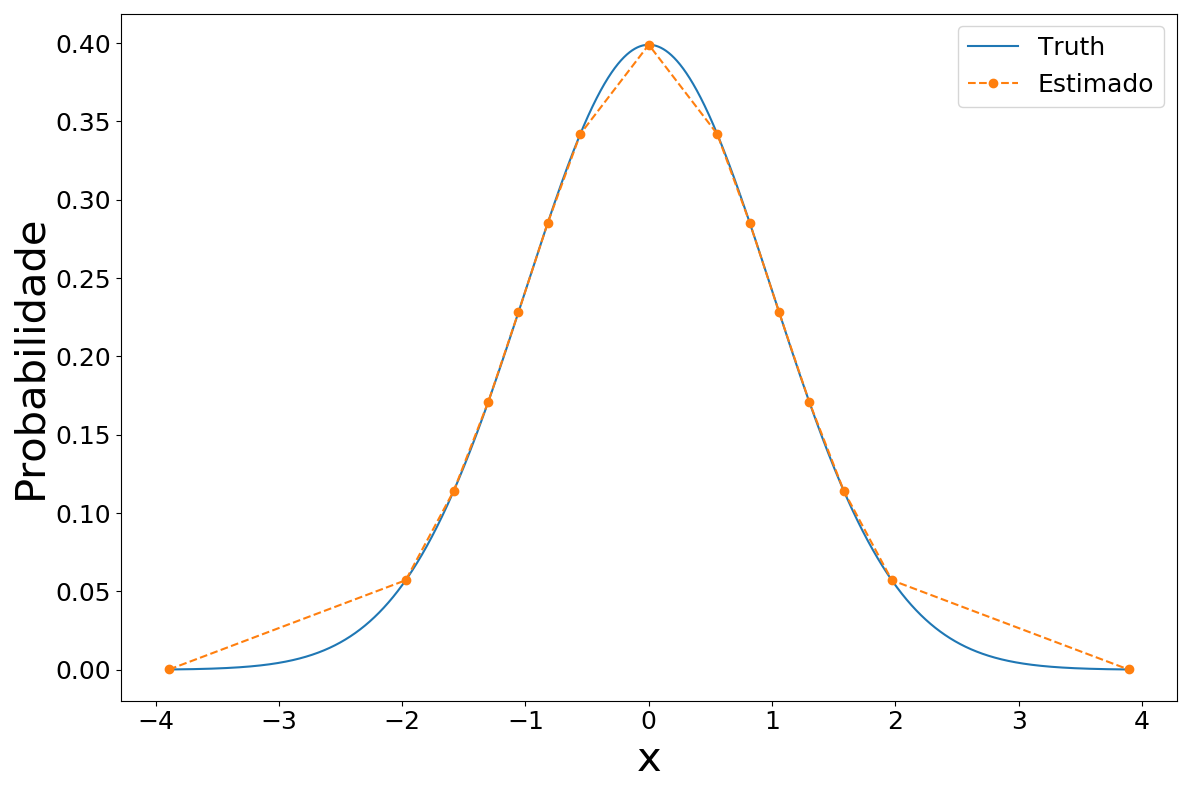
\includegraphics[width=\linewidth]{./figuras/PDFm_normal_15}
		\caption{}
		\label{fig:pdfnorm15}
	\end{subfigure}
	\hfill
	\begin{subfigure}[b]{0.45\textwidth}
		\centering 
		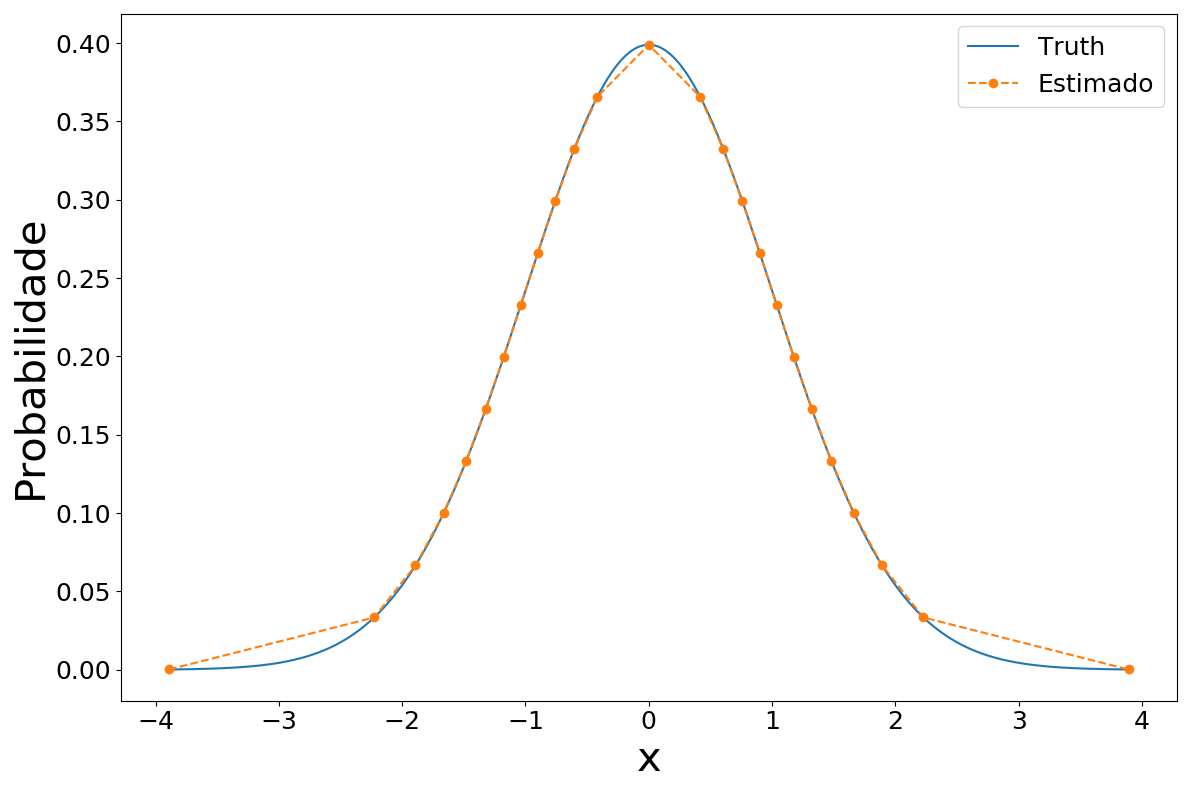
\includegraphics[width=\linewidth]{./figuras/PDFm_normal_25}
		\caption{}
		\label{fig:pdfnorm25}
	\end{subfigure}

	\begin{subfigure}[b]{0.45\textwidth}
		\centering 
		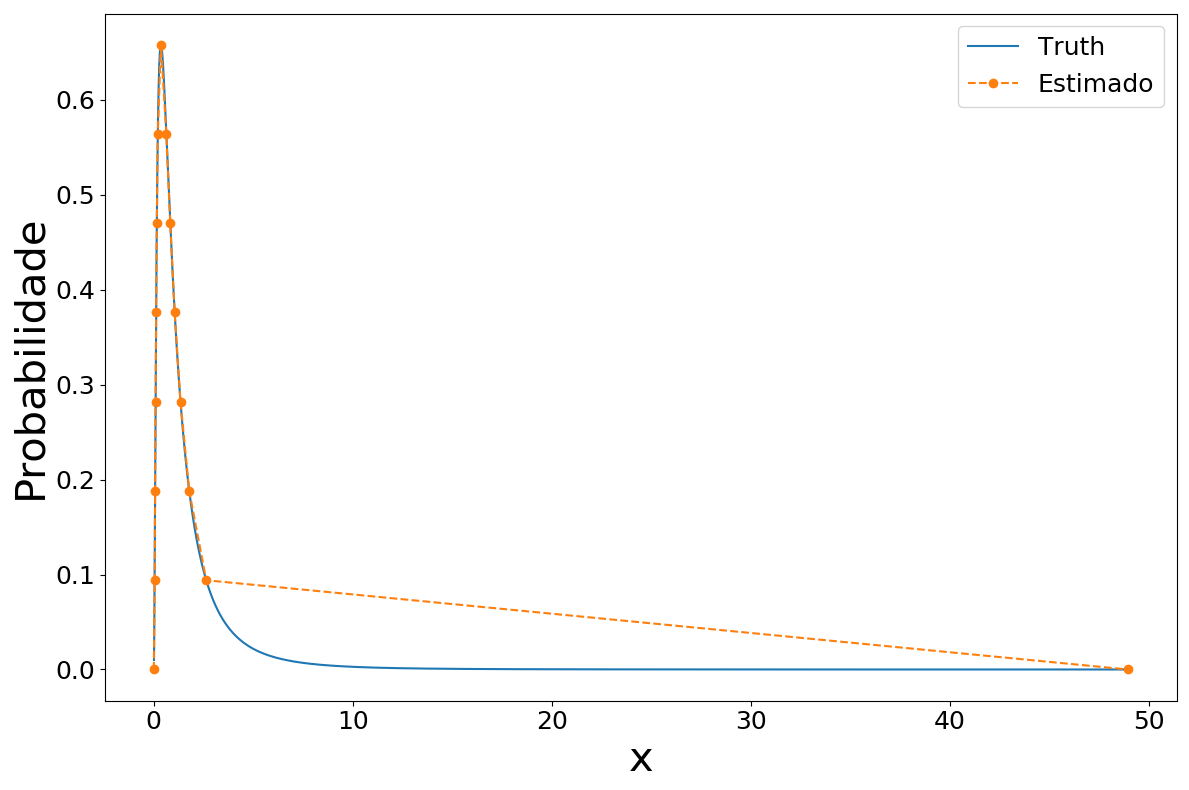
\includegraphics[width=\linewidth]{./figuras/PDFm_lognormal_15_1}
		\caption{}
		\label{fig:pdflognorm15}
	\end{subfigure}
	\hfill
	\begin{subfigure}[b]{0.45\textwidth}
		\centering 
		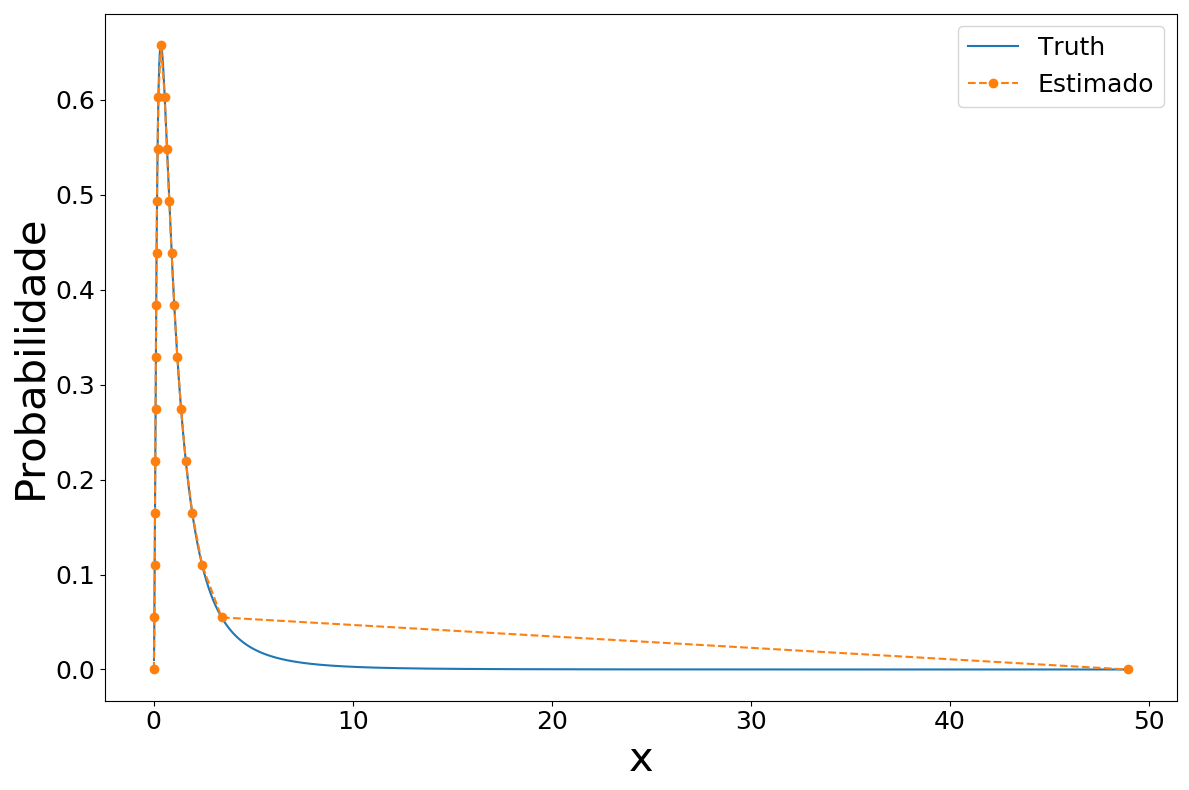
\includegraphics[width=\linewidth]{./figuras/PDFm_lognormal_25_1}
		\caption{}
		\label{fig:pdflognorm25}
	\end{subfigure}
	
	\caption{Discretização utilizando o método de \textit{PDFm}: (a) N(0,1) com $N = 15$, (b) N(0,1) com $N = 25$, (c) L(0,1) com $N = 15$ e (d) L(0,1) com $N = 25$.}
	\label{fig:pdfmnorm}
\end{figure}

Deste modo, este método relaciona os pontos positivos da \ac{CDFm} para regiões de alta probabilidade sendo que seu erro para as regiões de baixa probabilidade é um pouco menor.
%Deste modo este método possui pontos positivos e negativos dos dois métodos anteriormente apresentados, \textit{Linspace} e \ac{CDFm} sendo mais indicado para distribuições simétricas, como a Gaussiana.

\begin{figure}[H]
	\centering\begin{subfigure}[b]{0.45\textwidth}
		\centering 
		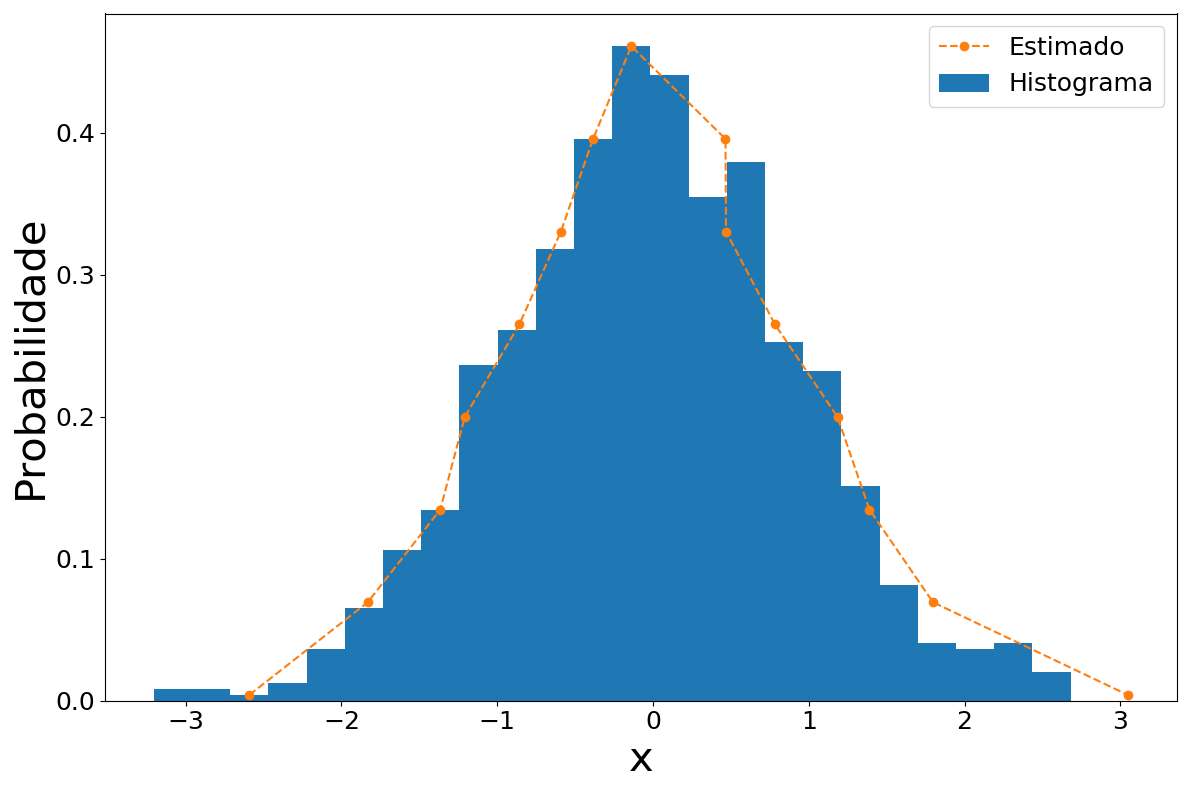
\includegraphics[width=\linewidth]{./figuras/PDFm_normal_15_1000_0}
		\caption{}
		\label{fig:pdfm_norm15_data}
	\end{subfigure}
	\hfill
	\begin{subfigure}[b]{0.45\textwidth}
		\centering 
		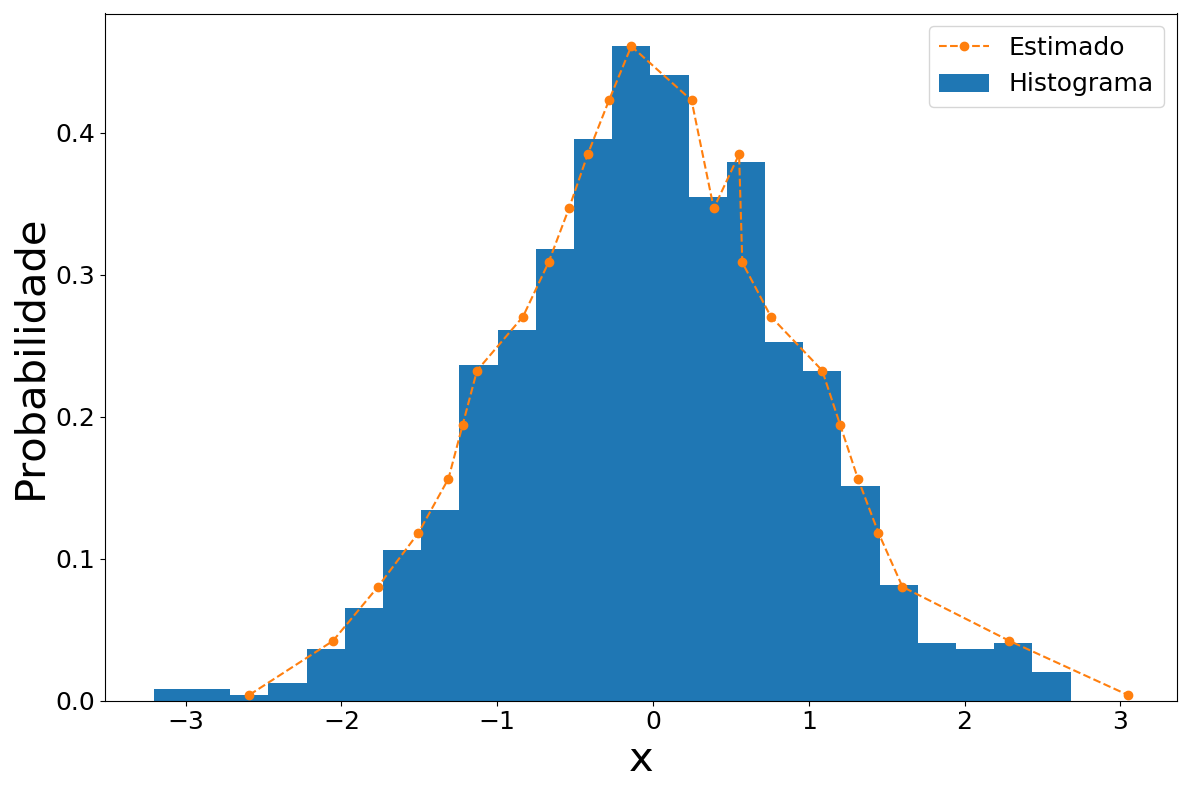
\includegraphics[width=\linewidth]{./figuras/PDFm_normal_25_1000_0}
		\caption{}
		\label{fig:pdfm_norm25_data}
	\end{subfigure}
	\\
	\begin{subfigure}[b]{0.45\textwidth}
		\centering 
		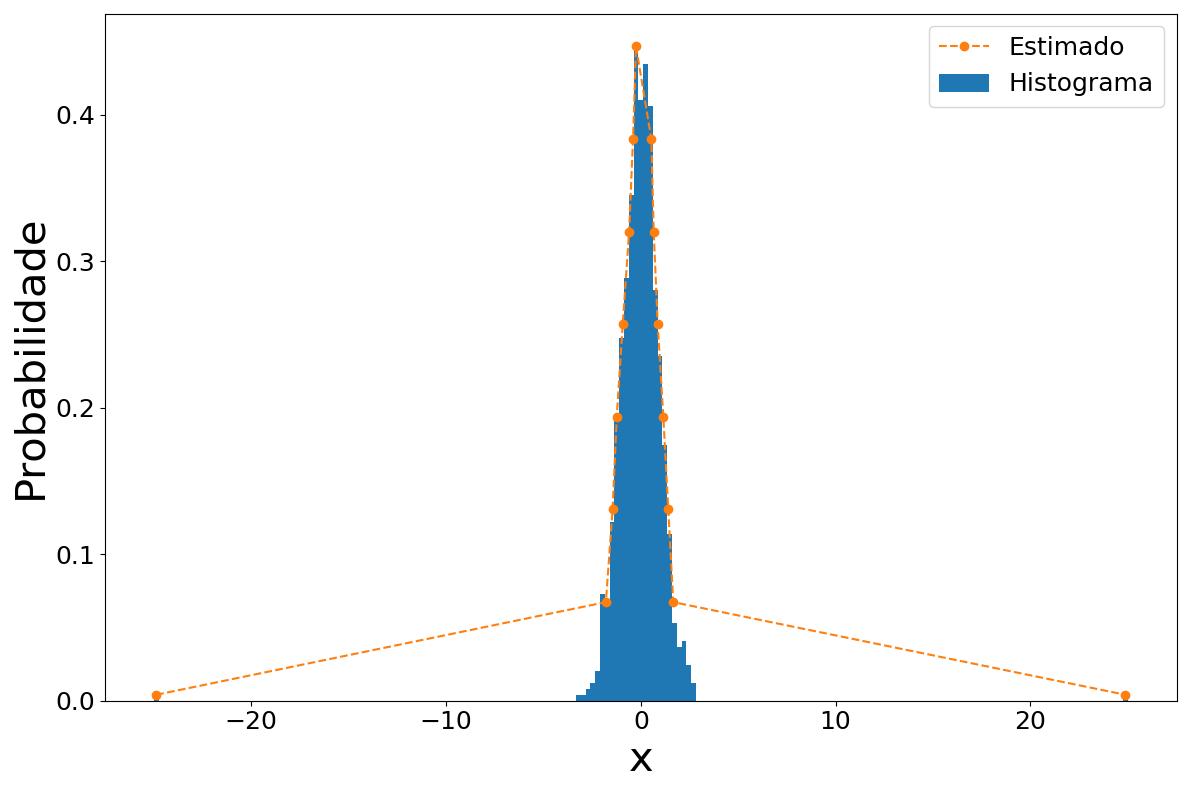
\includegraphics[width=\linewidth]{./figuras/PDFm_normal_15_1000_25}
		\caption{}
		\label{fig:pdfm_norm15_data_out}
	\end{subfigure}
	\hfill
	\begin{subfigure}[b]{0.45\textwidth}
		\centering 
		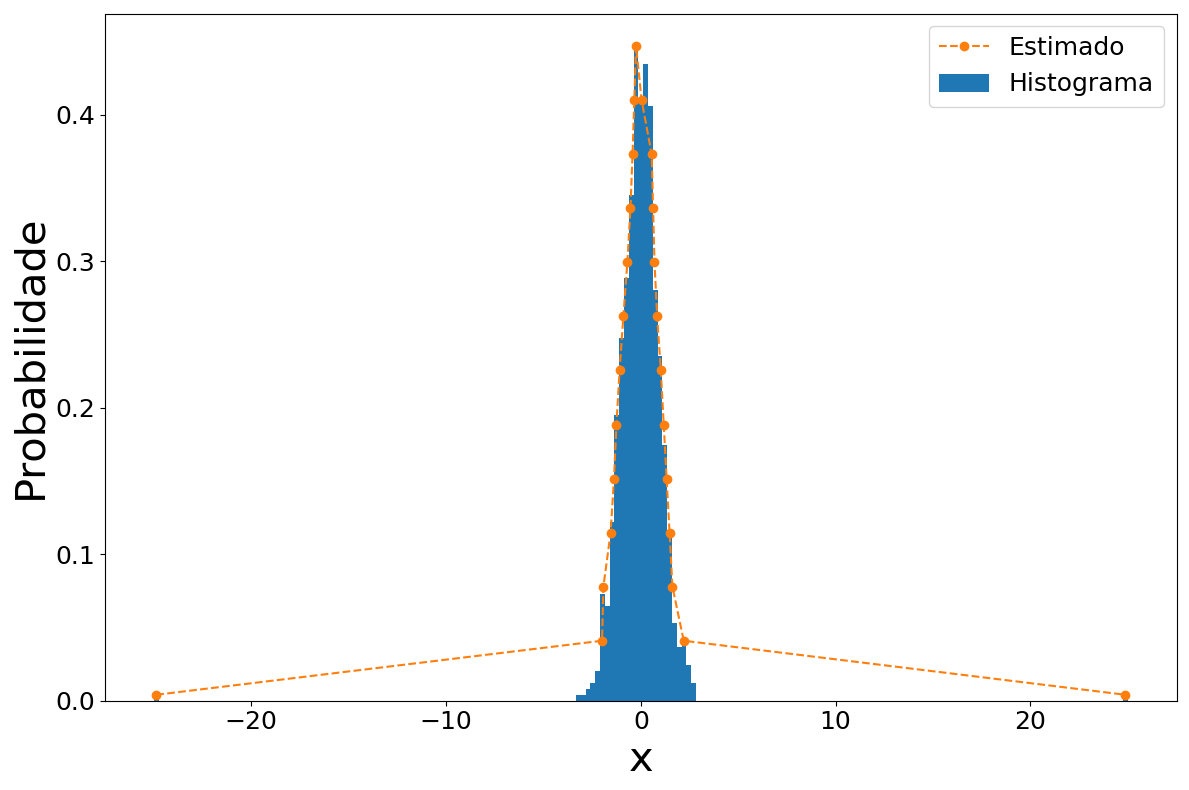
\includegraphics[width=\linewidth]{./figuras/PDFm_normal_25_1000_25}
		\caption{}
		\label{fig:pdfm_norm25_data_out}
	\end{subfigure}
	\\
	\begin{subfigure}[b]{0.45\textwidth}
		\centering 
		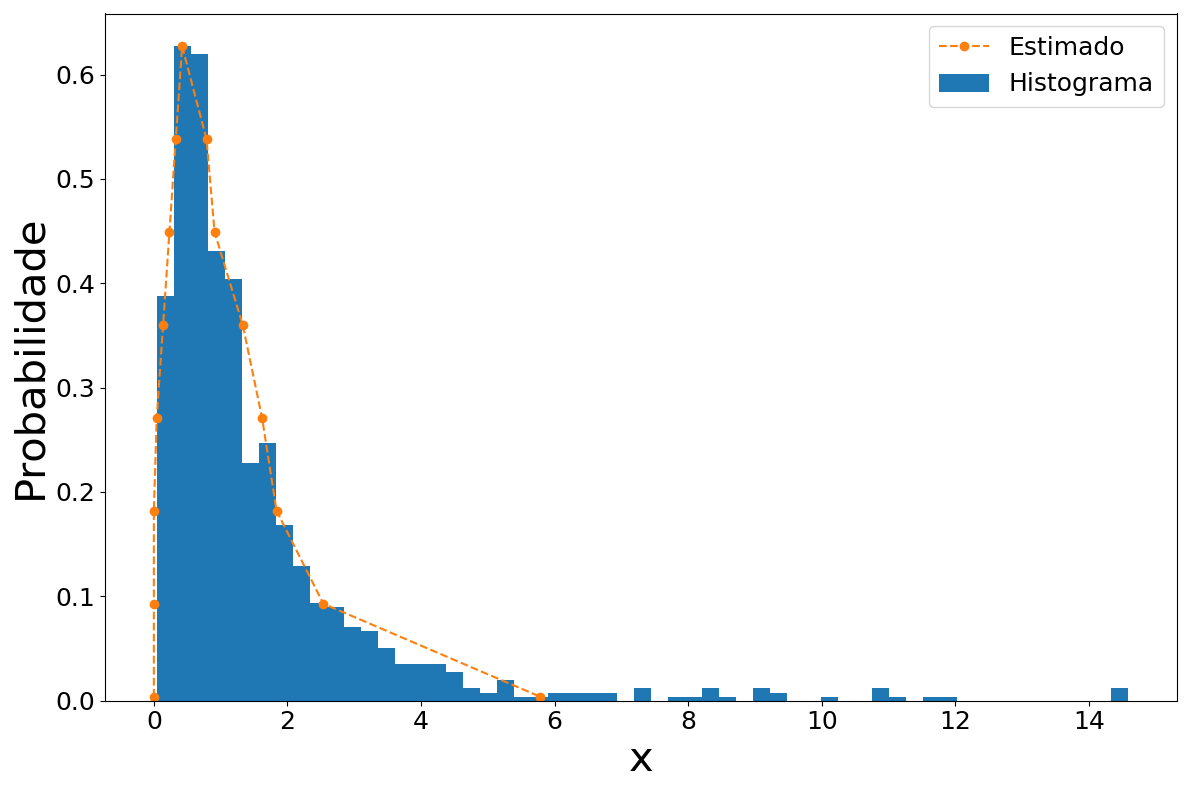
\includegraphics[width=\linewidth]{./figuras/PDFm_lognormal_15_1000_0}
		\caption{}
		\label{fig:pdfm_lognorm15_data}
	\end{subfigure}
	\hfill
	\begin{subfigure}[b]{0.45\textwidth}
		\centering 
		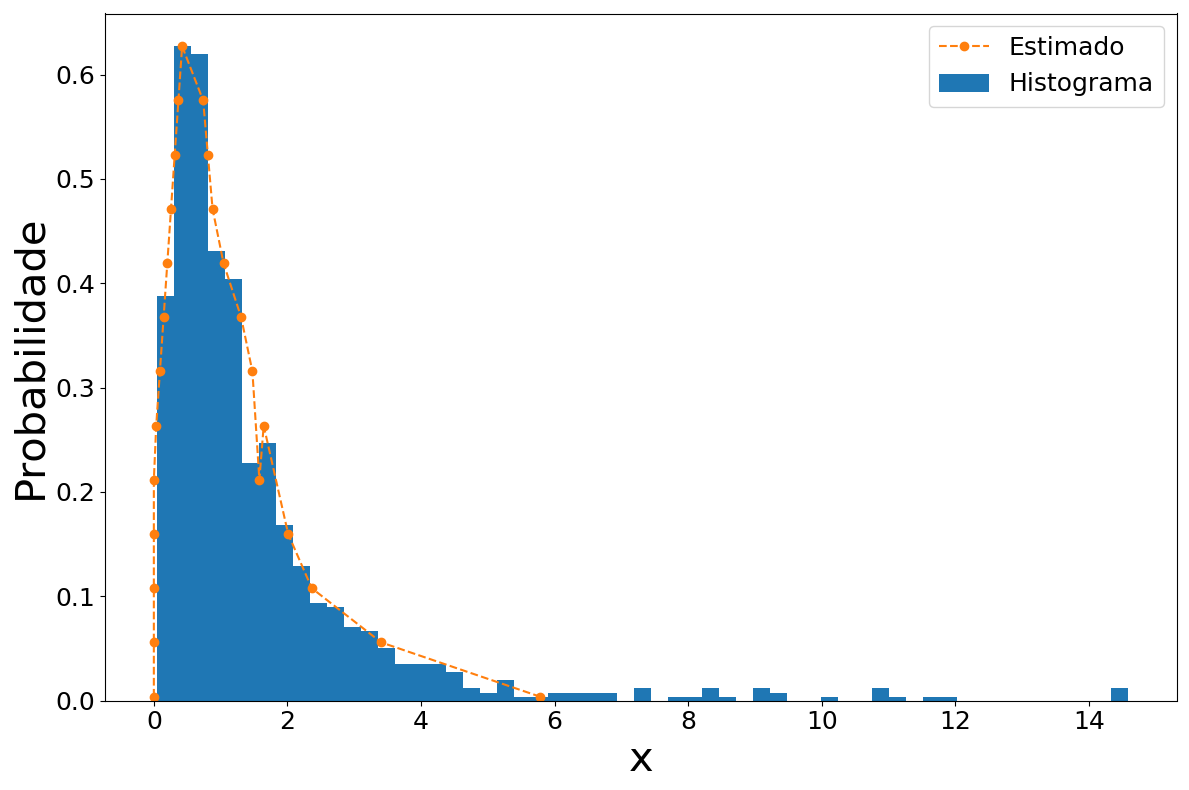
\includegraphics[width=\linewidth]{./figuras/PDFm_lognormal_25_1000_0}
		\caption{}
		\label{fig:pdfm_lognorm25_data}
	\end{subfigure}
	\caption{Discretização com os dados gerados utilizando o método \ac{PDFm}: (a) randN(0,1) com $N = 15$, (b) randN(0,1) com $N = 25$, (c) randN(0,1) com $N = 15$ e \textit{outlier} em $\pm 25$, (d) randN(0,1) com $N = 25$ e \textit{outlier} em $\pm 25$, (e) randL(0,1) com $ N = 15 $ e (f) randL(0,1) com $ N = 25 $.}
	\label{fig:pdfm_data}
\end{figure}

%Para a distribuição Normal, este método apresenta um maior erro na região de alta probabilidade do que o método \ac{CDFm} mas nas regiões de baixa probabilidade o erro de estimação é menor do que o visto anteriormente, fazendo assim uma combinação dos métodos \textit{Linspace} e \textit{CDFm}.
\subsection{Método \textit{iPDF1}}

Este método tem como base fazer a discretização baseada na primeira derivada, com isso é esperado uma melhor resolução nos pontos em que a variação da distribuição é maior, como pode ser verificado na Figura~\ref{fig:ipdfmnorm} e no Apêndice~\ref{cap:anexoiPDF1} em que este padrão também se repete. 

\begin{figure}[H]
	\centering
	\begin{subfigure}[b]{0.45\textwidth}
		\centering 
		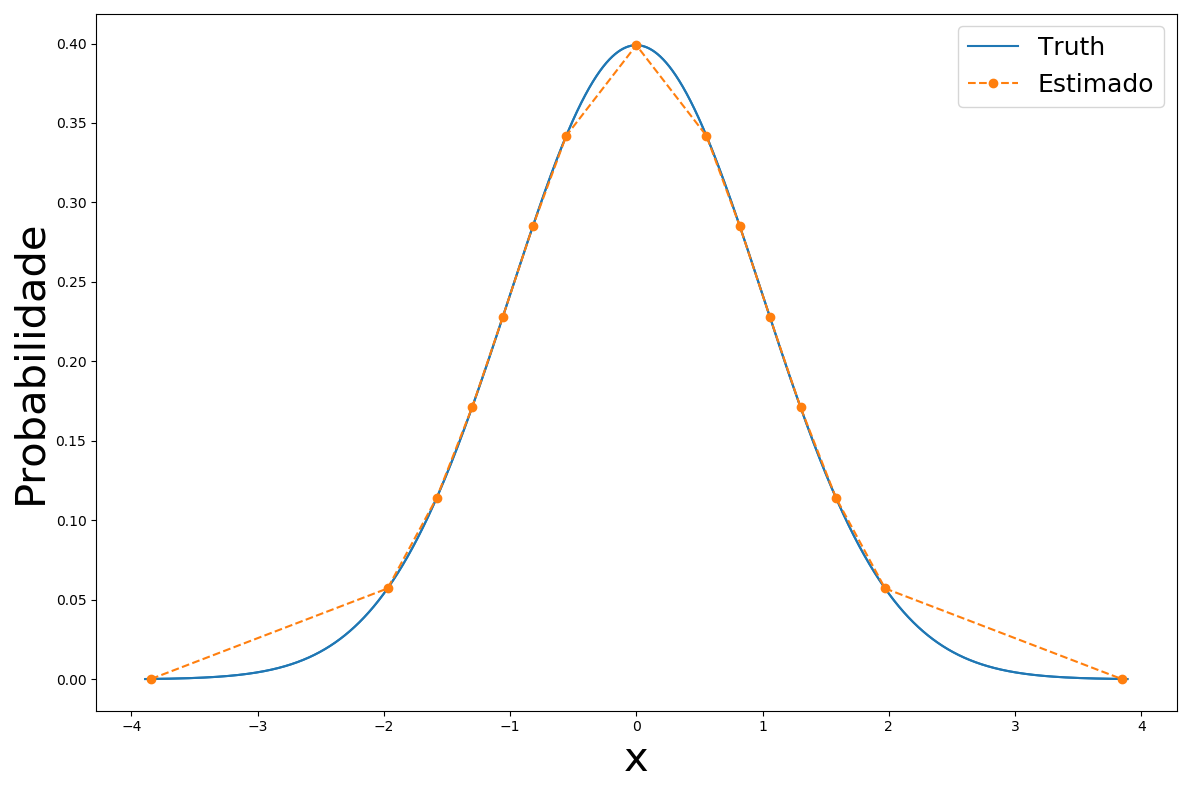
\includegraphics[width=\linewidth]{./figuras/iPDF1_normal_15}
		\caption{}
		\label{fig:ipdfnorm15}
	\end{subfigure}
	\hfill
	\begin{subfigure}[b]{0.45\textwidth}
		\centering 
		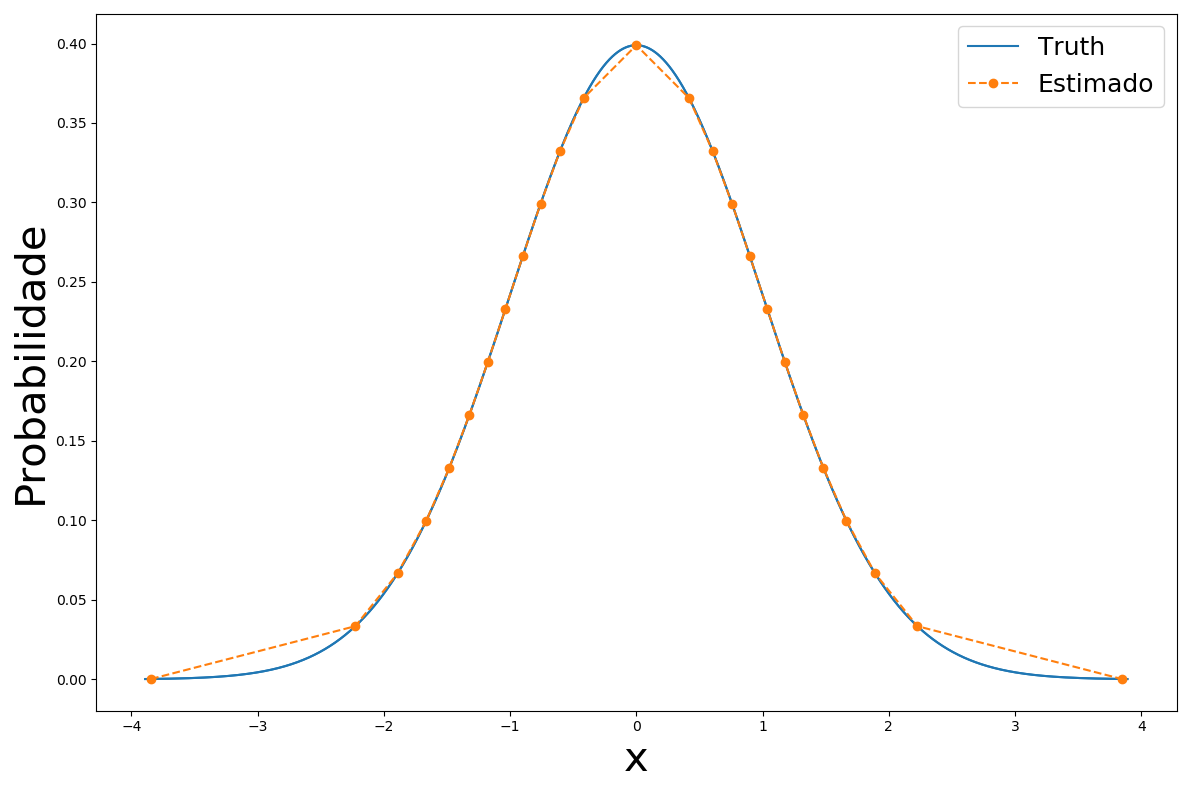
\includegraphics[width=\linewidth]{./figuras/iPDF1_normal_25}
		\caption{}
		\label{fig:ipdfnorm25}
	\end{subfigure}

	\begin{subfigure}[b]{0.45\textwidth}
		\centering 
		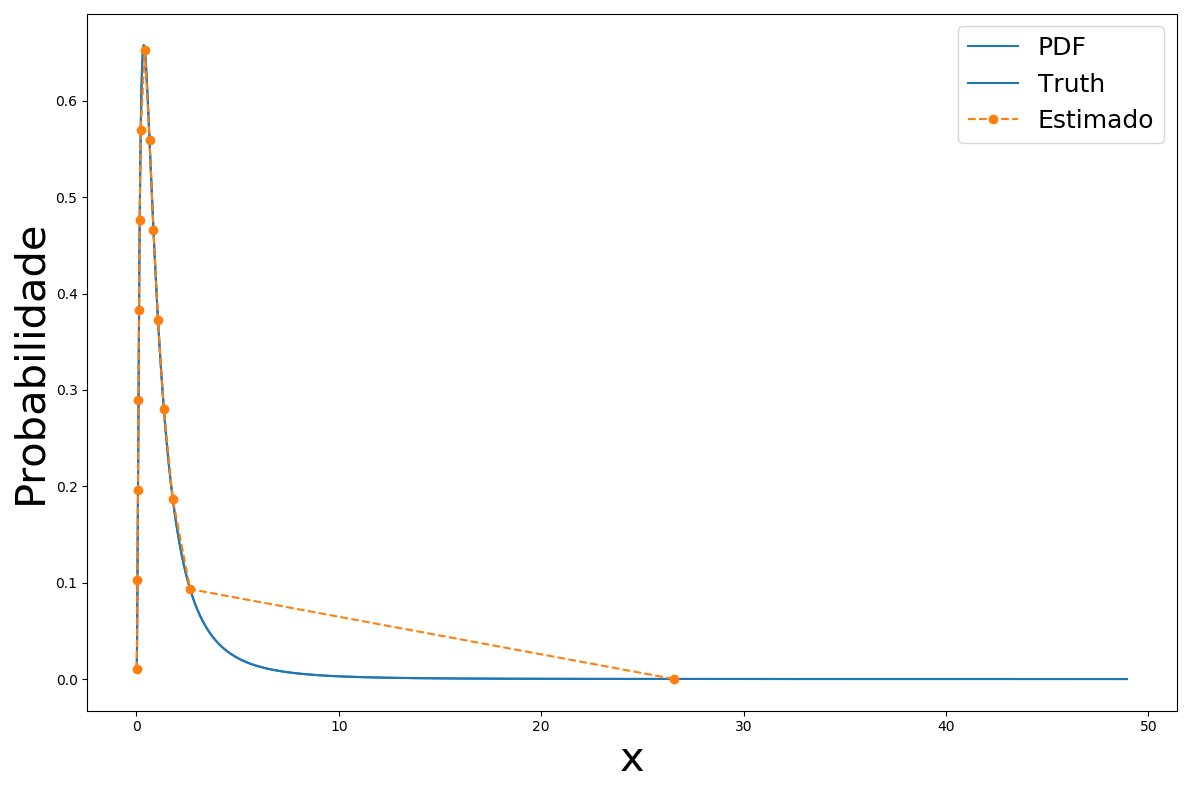
\includegraphics[width=\linewidth]{./figuras/iPDF1_lognormal_15}
		\caption{}
		\label{fig:ipdflognorm15}
	\end{subfigure}
	\hfill
	\begin{subfigure}[b]{0.45\textwidth}
		\centering 
		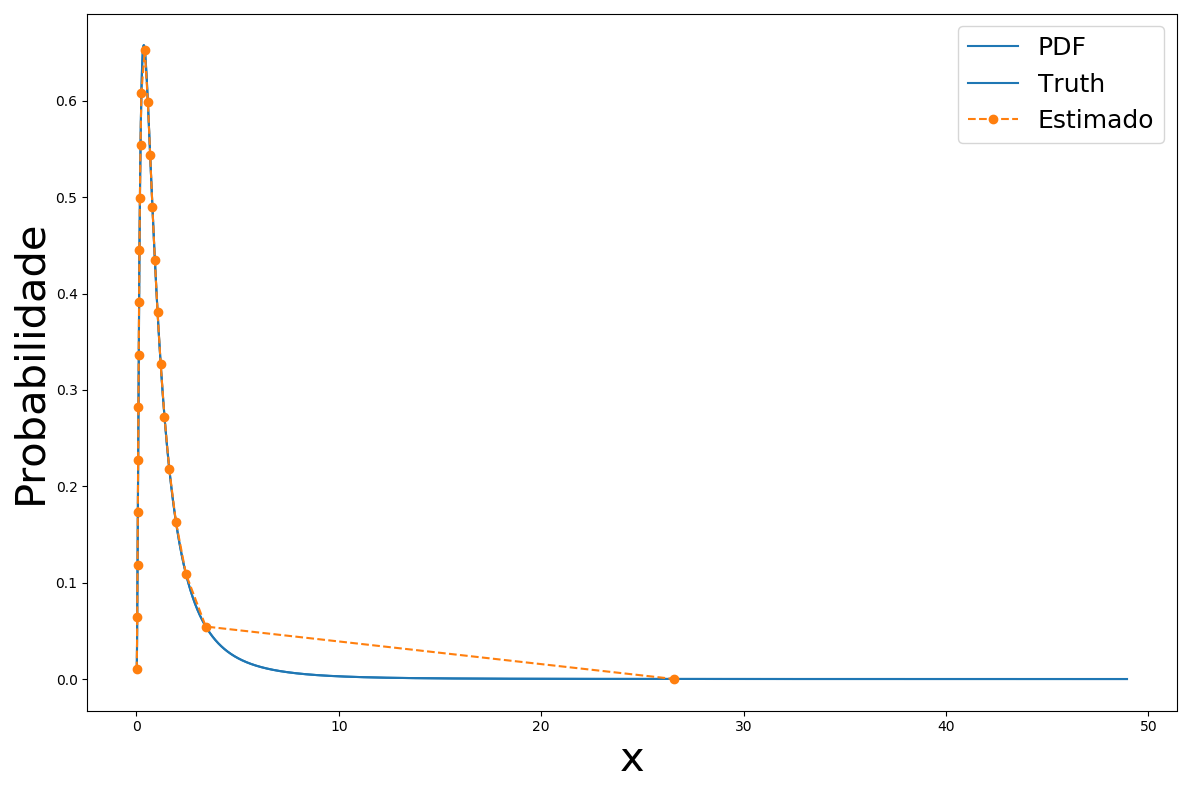
\includegraphics[width=\linewidth]{./figuras/iPDF1_lognormal_25}
		\caption{}
		\label{fig:ipdflognorm25}
	\end{subfigure}
	
	\caption{Discretização utilizando o método de \textit{iPDF1}: (a) N(0,1) com $N = 15$, (b) N(0,1) com $N = 25$, (c) L(0,1) com $N = 15$ e (d) L(0,1) com $N = 25$.}
	\label{fig:ipdfmnorm}
\end{figure}

Já para os dados gerados, devido ao fato de sua derivada discreta inserir ruido, sua CDF acaba sendo suavizada, fazendo com que este coloque mais pontos na região de baixa probabilidade, como pode ser visto na Figura~\ref{fig:ipdf1_data} e, em especial nas Figuras~\ref{fig:ipdf1_norm15_data_out} e \ref{fig:ipdf1_norm25_data_out} em que o erro na calda é baixo.

\begin{figure}[H]
	\centering\begin{subfigure}[b]{0.45\textwidth}
		\centering 
		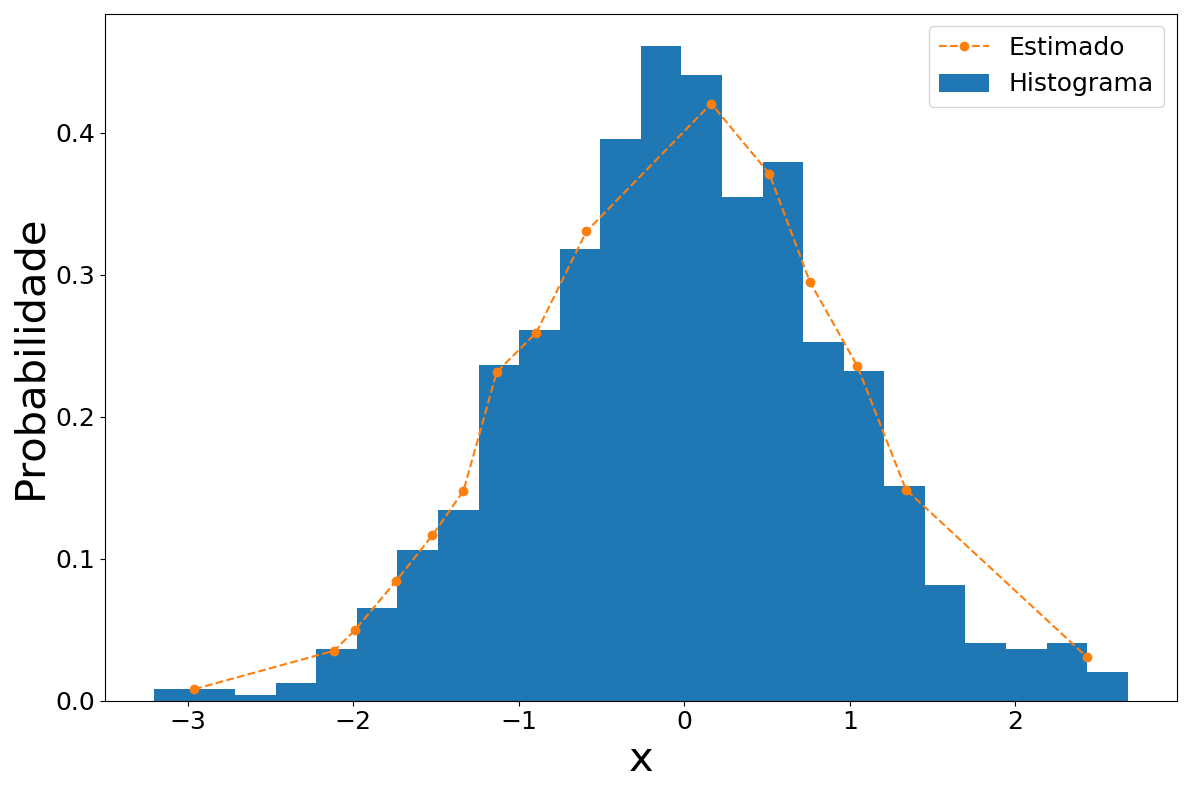
\includegraphics[width=\linewidth]{./figuras/iPDF1_normal_15_1_1000_0}
		\caption{}
		\label{fig:ipdf1_norm15_data}
	\end{subfigure}
	\hfill
	\begin{subfigure}[b]{0.45\textwidth}
		\centering 
		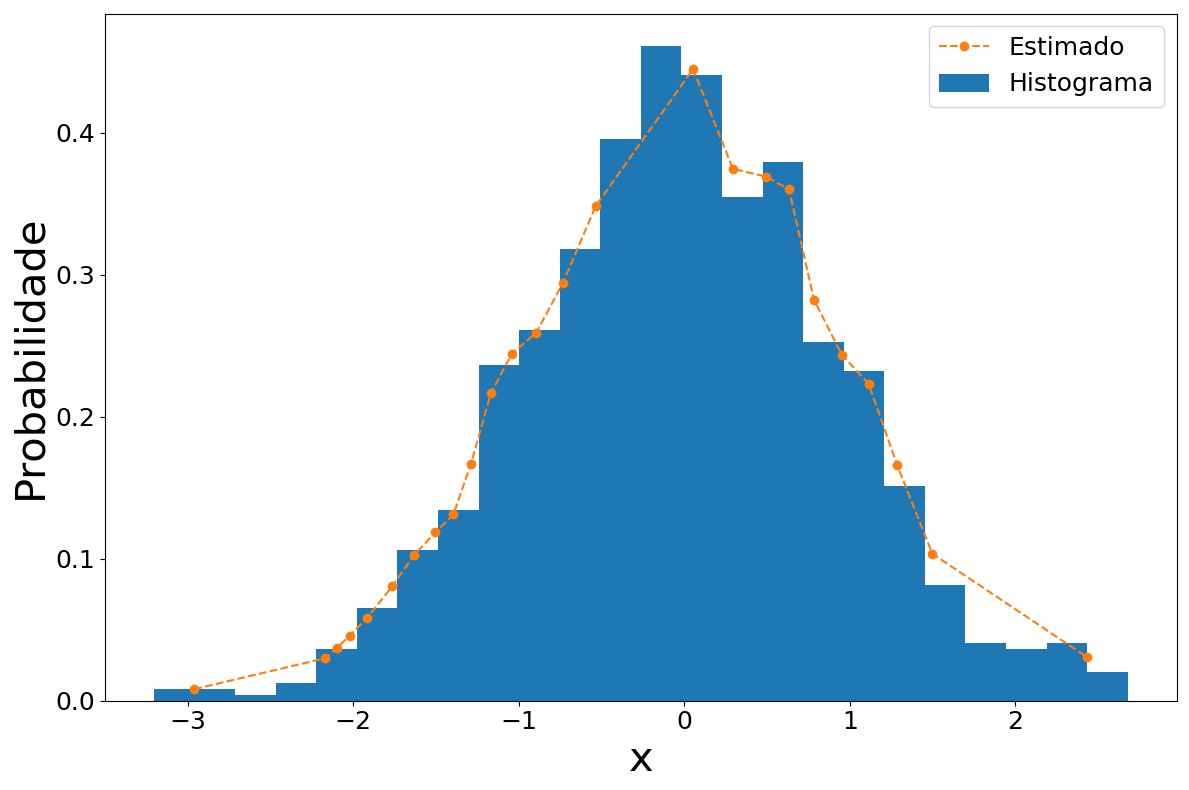
\includegraphics[width=\linewidth]{./figuras/iPDF1_normal_25_1_1000_0}
		\caption{}
		\label{fig:ipdf1_norm25_data}
	\end{subfigure}
	\\
	\begin{subfigure}[b]{0.45\textwidth}
		\centering 
		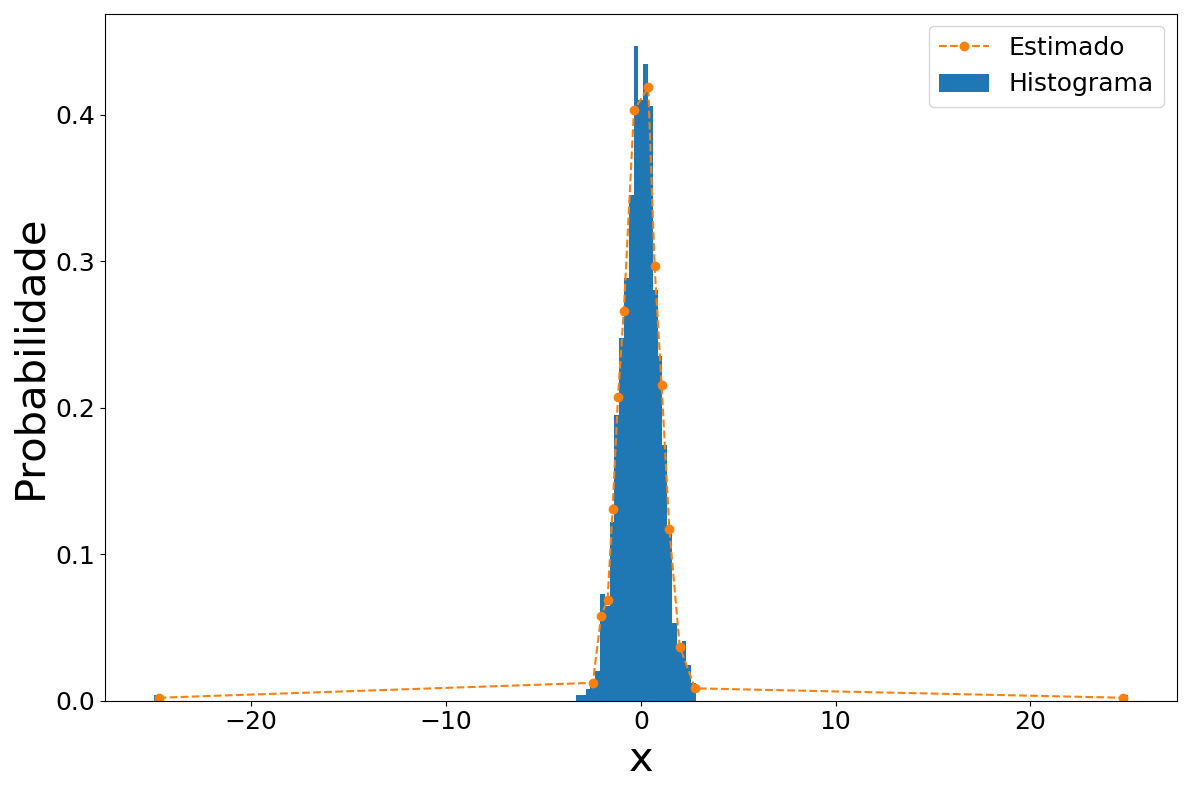
\includegraphics[width=\linewidth]{./figuras/iPDF1_normal_15_1_1000_25}
		\caption{}
		\label{fig:ipdf1_norm15_data_out}
	\end{subfigure}
	\hfill
	\begin{subfigure}[b]{0.45\textwidth}
		\centering 
		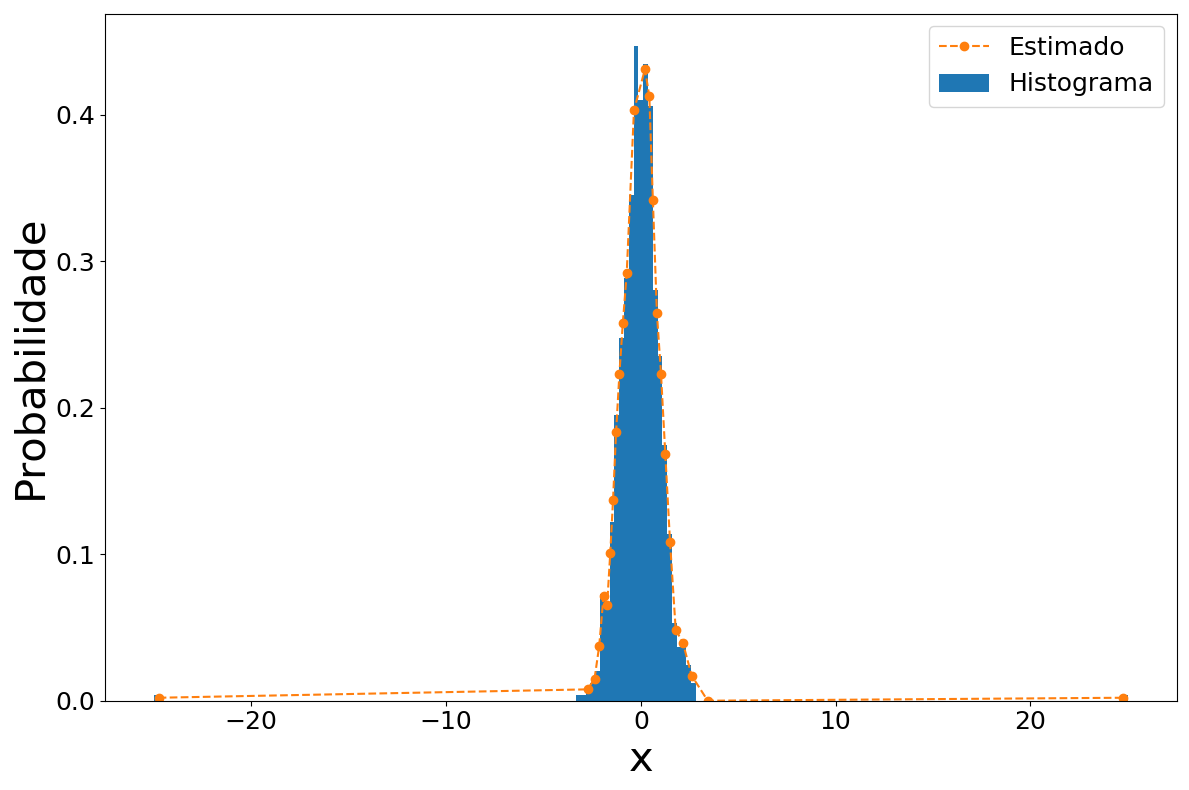
\includegraphics[width=\linewidth]{./figuras/iPDF1_normal_25_1_1000_25}
		\caption{}
		\label{fig:ipdf1_norm25_data_out}
	\end{subfigure}
	\\
	\begin{subfigure}[b]{0.45\textwidth}
		\centering 
		\includegraphics[width=\linewidth]{./figuras/iPDF1_lognormal_15_1_1000_0}
		\caption{}
		\label{fig:ipdf1_lognorm15_data}
	\end{subfigure}
	\hfill
	\begin{subfigure}[b]{0.45\textwidth}
		\centering 
		\includegraphics[width=\linewidth]{./figuras/iPDF1_lognormal_25_1_1000_0}
		\caption{}
		\label{fig:ipdf1_lognorm25_data}
	\end{subfigure}
	\caption{Discretização com os dados gerados utilizando o método \ac{iPDF1}: (a) randN(0,1) com $N = 15$, (b) randN(0,1) com $N = 25$, (c) randN(0,1) com $N = 15$ e \textit{outlier} em $\pm 25$, (d) randN(0,1) com $N = 25$ e \textit{outlier} em $\pm 25$, (e) randL(0,1) com $ N = 15 $ e (f) randL(0,1) com $ N = 25 $.}
	\label{fig:ipdf1_data}
\end{figure}


\subsection{Método \textit{iPDF2}}

A \ac{iPDF2} se baseia na segunda derivada, com isso, é esperado que o número de pontos seja maior onde haja uma variação de sua derivada e menor nos pontos de inflexão, como é mostrado na Figura~\ref{fig:ipdf2norm15} e \ref{fig:ipdf2norm25}. O mesmo acontece para as Figuras~\ref{fig:ipdf2_lognorm15_data} e \ref{fig:ipdf2_lognorm25_data}, mas, como a taxa de variação é muito maior na porção esquerda da distribuição, a quantidade de pontos do lado direito fica reduzido, fazendo com que o erro de estimação aumente.

\begin{figure}[H]
	\centering
	\begin{subfigure}[b]{0.45\textwidth}
		\centering 
		\includegraphics[width=\linewidth]{./figuras/iPDF2_normal_15_1_0_0}
		\caption{}
		\label{fig:ipdf2norm15}
	\end{subfigure}
	\hfill
	\begin{subfigure}[b]{0.45\textwidth}
		\centering 
		\includegraphics[width=\linewidth]{./figuras/iPDF2_normal_25_1_0_0}
		\caption{}
		\label{fig:ipdf2norm25}
	\end{subfigure}

	\begin{subfigure}[b]{0.45\textwidth}
		\centering 
		\includegraphics[width=\linewidth]{./figuras/iPDF2_lognormal_25_1_0_0}
		\caption{}
		\label{fig:ipdf2lognorm15}
	\end{subfigure}
	\hfill
	\begin{subfigure}[b]{0.45\textwidth}
		\centering 
		\includegraphics[width=\linewidth]{./figuras/iPDF2_lognormal_25_1_0_0}
		\caption{}
		\label{fig:ipdf2lognorm25}
	\end{subfigure}
	
	\caption{Discretização utilizando o método de \textit{iPDF2}: (a) N(0,1) com $N = 15$, (b) N(0,1) com $N = 25$, (c) L(0,1) com $N = 15$ e (d) L(0,1) com $N = 25$.}
	\label{fig:ipdf2norm}
\end{figure}

Para os dados gerados, o mesmo problema ocorre no método \ac{iPDF1} só que com mais ruido, devido ao fato de ser a segunda derivada discreta, com isso a sua CDF é ainda mais suave, fazendo com que haja mais pontos na região de baixa probabilidade, diminuindo assim seu erro nessa região, mas aumentando na região onde a probabilidade é maior, conforme pode ser visto na Figura~\ref{fig:ipdf2_data}.

\begin{figure}[H]
	\centering\begin{subfigure}[b]{0.45\textwidth}
		\centering 
		\includegraphics[width=\linewidth]{./figuras/iPDF2_normal_15_1_1000_0}
		\caption{}
		\label{fig:ipdf2_norm15_data}
	\end{subfigure}
	\hfill
	\begin{subfigure}[b]{0.45\textwidth}
		\centering 
		\includegraphics[width=\linewidth]{./figuras/iPDF2_normal_25_1_1000_0}
		\caption{}
		\label{fig:ipdf2_norm25_data}
	\end{subfigure}
	\\
	\begin{subfigure}[b]{0.45\textwidth}
		\centering 
		\includegraphics[width=\linewidth]{./figuras/iPDF2_normal_15_1_1000_25}
		\caption{}
		\label{fig:ipdf2_norm15_data_out}
	\end{subfigure}
	\hfill
	\begin{subfigure}[b]{0.45\textwidth}
		\centering 
		\includegraphics[width=\linewidth]{./figuras/iPDF2_normal_25_1_1000_25}
		\caption{}
		\label{fig:ipdf2_norm25_data_out}
	\end{subfigure}
	\\
	\begin{subfigure}[b]{0.45\textwidth}
		\centering 
		\includegraphics[width=\linewidth]{./figuras/iPDF2_lognormal_15_1_1000_0}
		\caption{}
		\label{fig:ipdf2_lognorm15_data}
	\end{subfigure}
	\hfill
	\begin{subfigure}[b]{0.45\textwidth}
		\centering 
		\includegraphics[width=\linewidth]{./figuras/iPDF2_lognormal_25_1_1000_0}
		\caption{}
		\label{fig:ipdf2_lognorm25_data}
	\end{subfigure}
	\caption{Discretização com os dados gerados utilizando o método \ac{iPDF2}: (a) randN(0,1) com $N = 15$, (b) randN(0,1) com $N = 25$, (c) randN(0,1) com $N = 15$ e \textit{outlier} em $\pm 25$, (d) randN(0,1) com $N = 25$ e \textit{outlier} em $\pm 25$, (e) randL(0,1) com $ N = 15 $ e (f) randL(0,1) com $ N = 25 $.}
	\label{fig:ipdf2_data}
\end{figure}


\section{Custo Computacional}

Os algoritmo de \textit{Kernel} são muito utilizados na literatura no contexto de análise de dados ou modelagem de dados, entretanto é sabido que esse método é computacionalmente mais lento em comparação com outros. Por isso muitos pesquisadores fazem uso de algoritmos que efetuam aproximações matemáticas no intuito de ganhar em custo computacional, chamados de \textit{FastKDE}, ou seja, existe um \textit{trade-off} entre estabilidade numérica e economia computacional. Entretanto, como já mencionado, o tempo de processamento esta diretamente ligado ao número de eventos da distribuição e ao número de pontos a serem estimados.

Portanto, no intuito de ilustrar a consequência de se aumentar o número de pontos de estimação a Figura \ref{fig:compKDE} apresentada o tempo de processamento de um algoritmo matricial de \textit{FastKDE} utilizado para a estimação de uma distribuição gaussiana $N(0,1)$ ao se variar o número de eventos e número de pontos de estimação.

\begin{figure}[!ht]
	\centering
	\includegraphics[width=0.8\linewidth]{./figuras/custocomp.png}\\
	\caption{Gráfico do tempo de processamento de um algoritmo de estimação de densidades baseado em KDE quando aumenta-se o número de eventos a serem estimados e o número de pontos de estimação.}
	\label{fig:compKDE}
\end{figure}

Pode-se observar que o tempo de processamento para $N = 1024$ é aproximadamente $75\%$ maior que para $N = 128$ quando o número de eventos é igual a $10^5$ e aproximadamente $67\%$ maior para número de eventos igual a $10^4$. Ou seja, um método de discretização capaz de apresentar o mesmo erro de estimação mesmo com menos pontos de estimação pode trazer benefícios importantes em ambientes de alta exigência.


\section{Ambiente de Análise}

Para analisar as diferenças entre a \ac{PDF} real e estimada ao longo de toda a extensão do eixo das abscissas, a área entre as duas \ac{PDF}s será usada como medida da estimação de erro. Além do mais, o eixo das abscissas foi dividida em $N$ regiões de mesmo tamanho, chamado \ac{RoI} \cite{ron1999art}. Essas regiões são compreendidas entre valores máximos e mínimos predefinidos do eixo horizontal. A Figura~\ref{fig:error} mostra este processo quando a abscissa é dividida em 20 regiões, todas compreendidas entre os valores $-4$ e $4$ do eixo $ x $.


\begin{figure}[!ht]
	\centering
	\includegraphics[width=0.6\linewidth]{./figuras/error1}\\
	\caption{Ilustração da medida de erro entre a PDF Real e a Estimada com 20 regiões de interesse.}
	\label{fig:error}
\end{figure}


A maneira que a \ac{RoI} é usada neste trabalho permitirá avaliar o erro de estimação em função de quatro diferentes parâmetros: Probabilidade; Eixo das abscissas; Primeira e Segunda Derivada. Para estimar os valores entre os pontos discretos, dois métodos de interpolação serão usados: interpolação pelo Vizinho Mais Próximo e Linear. 200 amostras serão usadas no processo de discretização. O erro de estimação tende a melhoras conforme o número de amostras aumenta mas sua característica geral não muda. Este último é a principal preocupação deste trabalho. 
